\documentclass{article}
\usepackage{graphicx} % Required for inserting images
\usepackage{pgfplots}
%\pgfplotsset{compat=1.18}
\usepackage{amsmath}
\usepackage{amssymb}
\usepackage{amsfonts}
\usepackage{amsthm}
\usepackage{mathtools}
\usepackage{bm}

% Mathematics
\usepackage{amsmath}
\usepackage{amssymb}
\usepackage{amsfonts}
\usepackage{amsthm}
\usepackage{mathtools}
\usepackage{bm}
\usepackage{tcolorbox}

% Graphics
\usepackage{graphicx}

% TikZ
\usepackage{tikz}
\usetikzlibrary{
	arrows.meta,
	positioning,
	calc,
	shapes.geometric,
	shapes.misc,
	decorations.pathmorphing
}

% Better Tables (if needed)
\usepackage{booktabs}
\usepackage{array}
\usepackage{multirow}

% Page Layout
\usepackage[a4paper,margin=1in]{geometry}

% Hyperlinks
\usepackage{hyperref}

% Better Lists
\usepackage{enumitem}

% Colors (optional)
\usepackage{xcolor}

% Captions
\usepackage{caption}

% Float Control
\usepackage{float}

% Paragraph Spacing (optional)
\usepackage{setspace}
\onehalfspacing
\title{DL_Unit_3}
\author{sujit4uwbslg }
\date{August 2026}

\begin{document}
	
	
	%%%%%%%%%%%%%%%%%%%%%%%%%%%%%%%%%%%%%%%%%%%%%%%%%%%%%%%%%%%%%%%%%%%%%%
	\section{Autoencoder}
	
	An autoencoder is a special type of feed-forward neural network.
	
	\begin{figure}[!ht]
		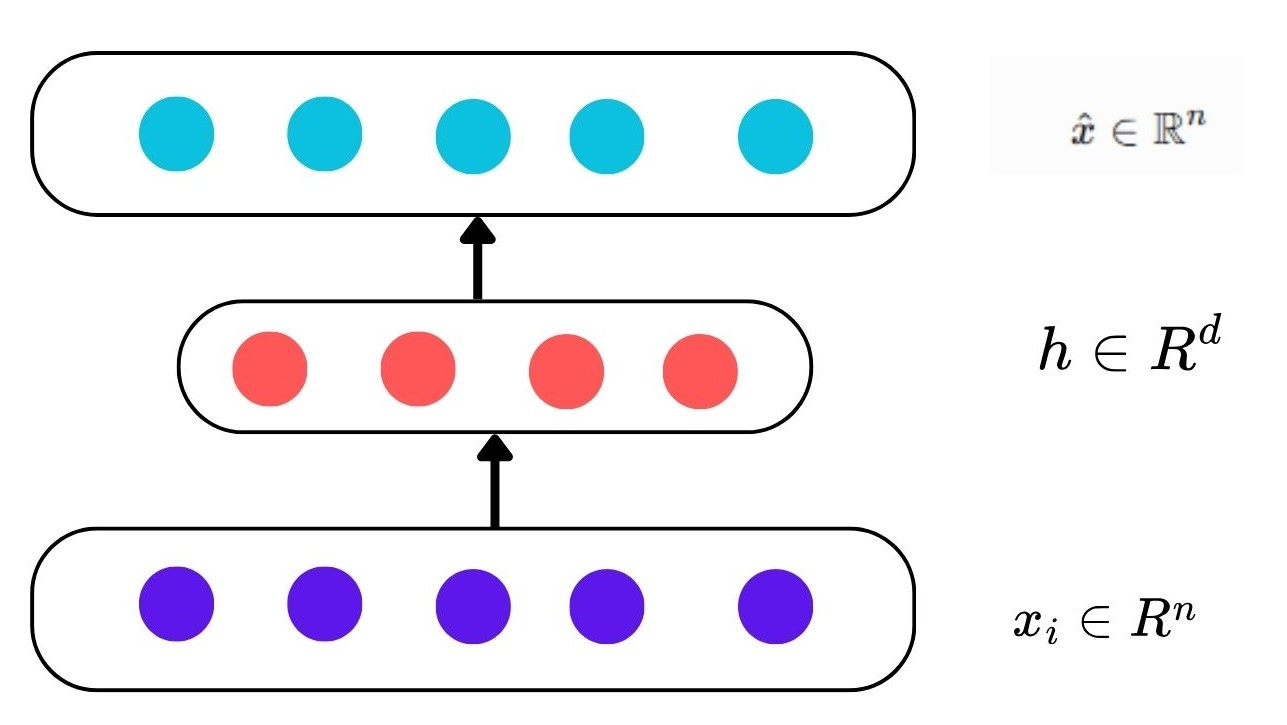
\includegraphics[width=0.5\linewidth]{images/autoencoder_architecture_1.jpg}
	\end{figure}
	
	\begin{enumerate}
		\item \textbf{Encoder}
		
		The encoder maps the input \(x_i\) into a hidden representation \(h\).
		
		\[
		x_i\in\mathbb{R}^{p}
		\]
		
		\[
		\Downarrow\;W
		\]
		
		\[
		h\in\mathbb{R}^{d}
		\]
		
		\[
		\Downarrow\;W'
		\]
		
		\[
		\hat{x}_i\in\mathbb{R}^{p}
		\]
		
		The hidden representation is
		
		\[
		\boxed{h=g(Wx_i+b)}
		\]
		
		where
		
		\begin{itemize}
			\item \(W\) : encoder weight matrix,
			\item \(b\) : bias vector,
			\item \(g(\cdot)\) : activation function.
		\end{itemize}
		
		\bigskip
		
		\begin{center}
			\begin{tikzpicture}[>=latex,scale=1]
				
				% Input layer
				\foreach \y in {2,1,0,-1,-2}
				{
					\draw (0,\y) circle (0.16);
				}
				
				\node at (0,-2.6) {$x_i\in\mathbb{R}^{p}$};
				
				% Hidden layer
				\foreach \y in {1,0,-1}
				{
					\draw (4,\y) circle (0.16);
				}
				
				\node at (4,-2.0) {$h\in\mathbb{R}^{d}$};
				
				% Output layer
				\foreach \y in {2,1,0,-1,-2}
				{
					\draw (8,\y) circle (0.16);
				}
				
				\node at (8,-2.6) {$\hat{x}_i\in\mathbb{R}^{p}$};
				
				\draw[->,thick] (0.5,0)--(3.3,0);
				\node at (2,0.4) {$W$};
				
				\draw[->,thick] (4.5,0)--(7.3,0);
				\node at (6,0.4) {$W'$};
				
			\end{tikzpicture}
		\end{center}
		
		\item \textbf{Decoder}
		
		The decoder reconstructs the original input from the hidden representation.
		
		\[
		\boxed{\hat{x}_i=f(W'h+c)}
		\]
		
		where
		
		\begin{itemize}
			\item \(W'\) : decoder weights,
			\item \(c\) : decoder bias,
			\item \(f(\cdot)\) : decoder activation.
		\end{itemize}
		
		\item The model is trained to minimize a loss function so that
		
		\[
		\hat{x}_i\approx x_i.
		\]
		
		\item Assume
		
		\[
		\dim(h)\le \dim(x_i).
		\]
		
		If we are still able to reconstruct the input accurately, then the hidden representation \(h\) is a nearly loss-free encoding of \(x_i\).
		
		It captures the important characteristics of the input.
	\end{enumerate}
	
	%%%%%%%%%%%%%%%%%%%%%%%%%%%%%%%%%%%%%%%%%%%%%%%%%%%%%%%%%%%%%%%%%%%%%%
	\subsection{Undercomplete and Overcomplete Autoencoder}
	
	If
	
	\[
	\boxed{\dim(h)<\dim(x_i)}
	\]
	
	the autoencoder is called an
	
	\[
	\boxed{\text{Undercomplete Autoencoder}.}
	\]
	
	Otherwise,
	
	
	\begin{figure}[!ht]
		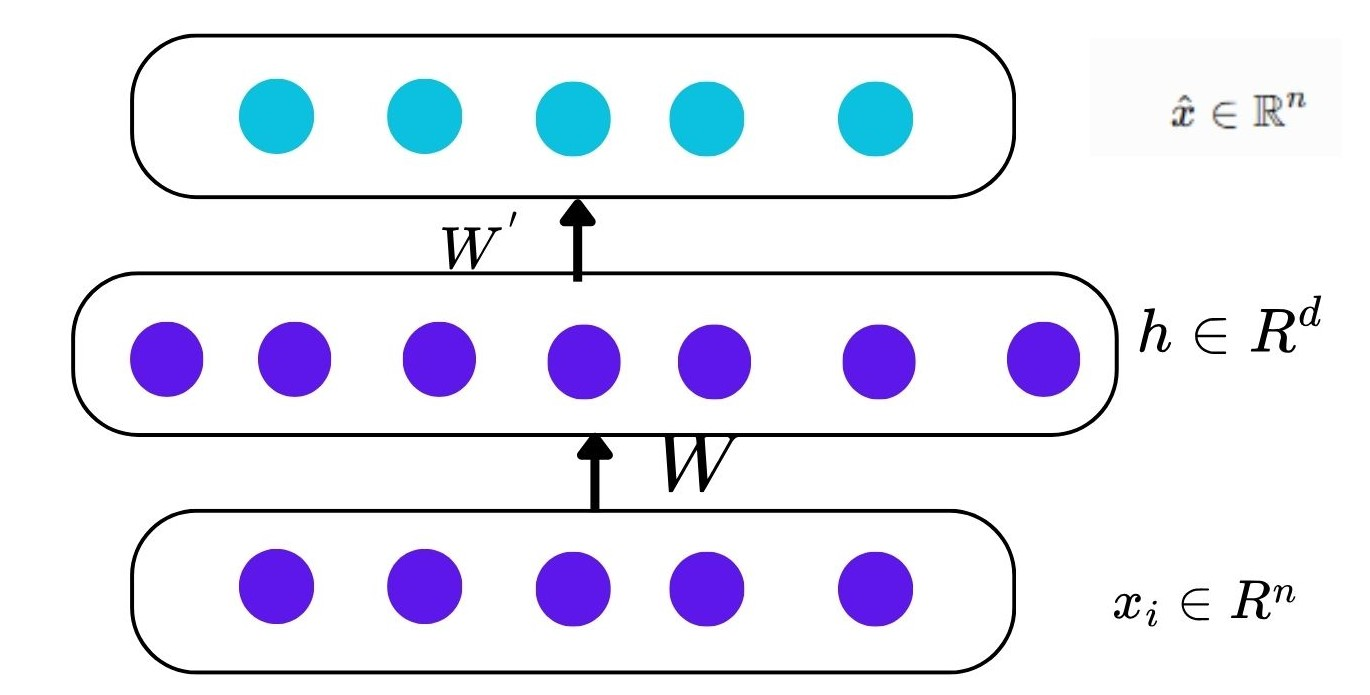
\includegraphics[width=0.7\linewidth]{images/OverCompleteAutoEncoder.jpg}
	\end{figure}
	
	\[
	\boxed{\dim(h)\ge \dim(x_i)}
	\]
	
	it becomes an
	
	\[
	\boxed{\text{Overcomplete Autoencoder}.}
	\]
	
	
	
	For an overcomplete autoencoder,
	
	\[
	\dim(h)\ge\dim(x_i),
	\]
	
	the network can learn the trivial identity mapping,
	
	\[
	x_i\longrightarrow h\longrightarrow \hat{x}_i,
	\]
	
	simply by copying the input into the hidden layer and copying it back.
	
	Such identity encoding is generally useless because it does not reveal the important characteristics of the data.
	
	Hence,
	
	\[
	\boxed{\dim(h)\ge\dim(x_i)}
	\]
	
	corresponds to an
	
	\[
	\boxed{\text{Overcomplete Autoencoder}.}
	\]
	
	Such encoders can easily memorize the training data.
	
	Therefore, additional constraints or regularization are required to prevent the network from learning the identity function.
	
	
	\section{Road Ahead: Autoencoder Design}
	
	To design an effective autoencoder, two important choices must be made:
	
	\begin{itemize}
		\item Choice of the encoder and decoder functions,
		\[
		g(\cdot),\qquad f(\cdot),
		\]
		\item Choice of the loss (objective) function.
	\end{itemize}
	
	We consider two categories of input data:
	
	\begin{enumerate}
		\item Binary-valued inputs
		\item Real-valued inputs
	\end{enumerate}
	
	%%%%%%%%%%%%%%%%%%%%%%%%%%%%%%%%%%%%%%%%%%%%%%%%%%%%%%%%%%%%%%
	
	\subsection*{Case 1: Binary Inputs}
	
	Suppose every input feature is binary,
	
	\[
	x_{ij}\in\{0,1\}.
	\]
	
	The encoder generates a hidden representation
	
	\[
	\mathbf{h}=g(W\mathbf{x}+b),
	\]
	
	and the decoder reconstructs the input.
	
	\begin{center}
		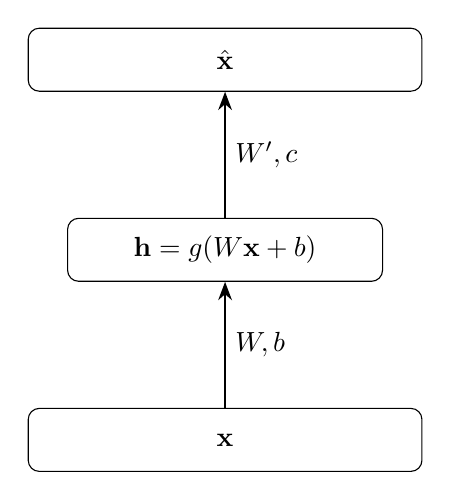
\begin{tikzpicture}[>=Stealth]
			
			\node[draw,rounded corners,minimum width=5cm,minimum height=0.8cm] (x)
			{$\mathbf{x}$};
			
			\node[draw,rounded corners,minimum width=4cm,minimum height=0.8cm,above=1.6cm of x] (h)
			{$\mathbf{h}=g(W\mathbf{x}+b)$};
			
			\node[draw,rounded corners,minimum width=5cm,minimum height=0.8cm,above=1.6cm of h] (xr)
			{$\hat{\mathbf{x}}$};
			
			\draw[->,thick] (x)--node[right]{$W,b$}(h);
			\draw[->,thick] (h)--node[right]{$W',c$}(xr);
			
		\end{tikzpicture}
	\end{center}
	
	Possible decoder choices are
	
	\[
	\hat{x}_i=\tanh(W'h+c),
	\]
	
	or
	
	\[
	\hat{x}_i=W'h+c,
	\]
	
	or
	
	\[
	\hat{x}_i=\sigma(W'h+c),
	\]
	
	where
	
	\[
	\sigma(z)=\frac{1}{1+e^{-z}}
	\]
	
	is the logistic sigmoid.
	
	Since the reconstructed output must lie between 0 and 1,
	
	\[
	0\le \hat{x}_i\le 1,
	\]
	
	the sigmoid decoder is the natural choice.
	
	%%%%%%%%%%%%%%%%%%%%%%%%%%%%%%%%%%%%%%%%%%%%%%%%%%%%%%%%%%%%%%
	
	\subsection*{Case 2: Real-Valued Inputs}
	
	Suppose the input consists of real-valued vectors,
	
	\[
	x_i\in\mathbb{R}^d.
	\]
	
	The decoder may be chosen as
	
	\[
	\hat{x}_i=\tanh(W'h+c),
	\]
	
	or
	
	\[
	\hat{x}_i=W'h+c,
	\]
	
	or
	
	\[
	\hat{x}_i=\sigma(W'h+c).
	\]
	
	Since the sigmoid function restricts the output to
	
	\[
	(0,1),
	\]
	
	it is generally unsuitable for reconstructing unrestricted real-valued data.
	
	Hence the linear decoder
	
	\[
	\boxed{\hat{x}=W'h+c}
	\]
	
	is generally preferred.
	
	%%%%%%%%%%%%%%%%%%%%%%%%%%%%%%%%%%%%%%%%%%%%%%%%%%%%%%%%%%%%%%
	
	\section{Choice of Loss Function}
	
	The objective of an autoencoder is to reconstruct the input as accurately as possible.
	
	That is,
	
	\[
	\hat{x}_i\approx x_i.
	\]
	
	The reconstruction error is measured using the Mean Squared Error (MSE)
	
	\[
	\boxed{
		J(W,W',b,c)
		=
		\frac1m
		\sum_{i=1}^{m}
		\sum_{j=1}^{d}
		(\hat{x}_{ij}-x_{ij})^2
	}
	\]
	
	or equivalently,
	
	\[
	\boxed{
		J
		=
		\frac1m
		\sum_{i=1}^{m}
		(\hat{x}_i-x_i)^T
		(\hat{x}_i-x_i)
	}
	\]
	
	where
	
	\[
	\hat{X}
	=
	\begin{bmatrix}
		\hat{x}_1^T\\
		\hat{x}_2^T\\
		\vdots\\
		\hat{x}_m^T
	\end{bmatrix},
	\qquad
	X
	=
	\begin{bmatrix}
		x_1^T\\
		x_2^T\\
		\vdots\\
		x_m^T
	\end{bmatrix}.
	\]
	
	%%%%%%%%%%%%%%%%%%%%%%%%%%%%%%%%%%%%%%%%%%%%%%%%%%%%%%%%%%%%%%
	
	\section{Training the Autoencoder}
	
	Training proceeds exactly like a standard feedforward neural network using backpropagation.
	
	The learnable parameters are
	
	\[
	\theta=\{W,W',b,c\}.
	\]
	
	The required gradients are
	
	\[
	\frac{\partial J}{\partial W},
	\qquad
	\frac{\partial J}{\partial W'},
	\qquad
	\frac{\partial J}{\partial b},
	\qquad
	\frac{\partial J}{\partial c}.
	\]
	
	%%%%%%%%%%%%%%%%%%%%%%%%%%%%%%%%%%%%%%%%%%%%%%%%%%%%%%%%%%%%%%
	
	\section{Neural Network Representation}
	
	\begin{center}
		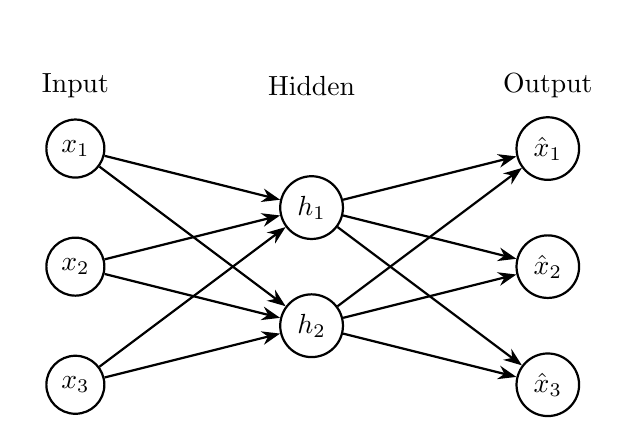
\begin{tikzpicture}[
			every node/.style={circle,draw,minimum size=7mm},
			>=Stealth,
			thick,
			scale=1.0
			]
			
			% Input layer
			\node (x1) at (0,0){$x_1$};
			\node (x2) at (0,-1.5){$x_2$};
			\node (x3) at (0,-3){$x_3$};
			
			% Hidden layer
			\node (h1) at (3,-0.75){$h_1$};
			\node (h2) at (3,-2.25){$h_2$};
			
			% Output layer
			\node (y1) at (6,0){$\hat{x}_1$};
			\node (y2) at (6,-1.5){$\hat{x}_2$};
			\node (y3) at (6,-3){$\hat{x}_3$};
			
			% Connections
			\foreach \i in {1,2,3}
			{
				\foreach \j in {1,2}
				{
					\draw[->](x\i)--(h\j);
				}
			}
			
			\foreach \i in {1,2}
			{
				\foreach \j in {1,2,3}
				{
					\draw[->](h\i)--(y\j);
				}
			}
			
			\node[draw=none] at (0,0.8){Input};
			\node[draw=none] at (3,0.8){Hidden};
			\node[draw=none] at (6,0.8){Output};
			
		\end{tikzpicture}
	\end{center}
	
	The forward computation is
	
	\[
	\boxed{
		h
		=
		g(Wx+b)
	}
	\]
	
	followed by
	
	\[
	\boxed{
		\hat{x}
		=
		f(W'h+c)
	}
	\]
	
	%%%%%%%%%%%%%%%%%%%%%%%%%%%%%%%%%%%%%%%%%%%%%%%%%%%%%%%%%%%%%%
	
	\section{Backpropagation}
	
	The reconstruction loss is
	
	\[
	J
	=
	(\hat{x}-x)^T(\hat{x}-x).
	\]
	
	Using the chain rule,
	
	\[
	\boxed{
		\frac{\partial J}{\partial W}
		=
		\frac{\partial J}{\partial a}
		\frac{\partial a}{\partial W}
	}
	\]
	
	where \(a\) denotes the pre-activation of a neuron.
	
	Similarly,
	
	\[
	\frac{\partial J}{\partial W'}
	=
	\frac{\partial J}{\partial \hat{x}}
	\frac{\partial \hat{x}}{\partial W'},
	\]
	
	\[
	\frac{\partial J}{\partial b}
	=
	\frac{\partial J}{\partial a}
	\frac{\partial a}{\partial b},
	\]
	
	and
	
	\[
	\frac{\partial J}{\partial c}
	=
	\frac{\partial J}{\partial \hat{x}}
	\frac{\partial \hat{x}}{\partial c}.
	\]
	
	The gradients are propagated backward layer by layer until every parameter has been updated.
	
	%%%%%%%%%%%%%%%%%%%%%%%%%%%%%%%%%%%%%%%%%%%%%%%%%%%%%%%%%%%%
	\section{Backpropagation for Mean Squared Error Loss}
	%%%%%%%%%%%%%%%%%%%%%%%%%%%%%%%%%%%%%%%%%%%%%%%%%%%%%%%%%%%%
	
	Recall that the reconstruction loss for a single training example is
	
	\[
	\mathcal{L}^{(\theta)}
	=
	(\hat{\mathbf{x}}_i-\mathbf{x}_i)^T
	(\hat{\mathbf{x}}_i-\mathbf{x}_i).
	\]
	
	Our objective is to compute
	
	\[
	\frac{\partial \mathcal{L}^{(\theta)}}{\partial W},
	\]
	
	using the chain rule.
	
	%%%%%%%%%%%%%%%%%%%%%%%%%%%%%%%%%%%%%%%%%%%%%%%%%%%%%%%%%%%%
	
	The derivative can be expanded as
	
	\[
	\boxed{
		\frac{\partial \mathcal{L}^{(\theta)}}{\partial W}
		=
		\frac{\partial \mathcal{L}^{(\theta)}}{\partial h}
		\;
		\frac{\partial h}{\partial a}
		\;
		\frac{\partial a}{\partial W}
	}
	\]
	
	where
	
	\[
	a=Wx+b.
	\]
	
	For a multi-layer network,
	
	\[
	\boxed{
		\frac{\partial \mathcal{L}^{(\theta)}}{\partial W}
		=
		\frac{\partial \mathcal{L}^{(\theta)}}{\partial h_2}
		\;
		\frac{\partial h_2}{\partial a_2}
		\;
		\frac{\partial a_2}{\partial h_1}
		\;
		\frac{\partial h_1}{\partial a_1}
		\;
		\frac{\partial a_1}{\partial W}
	}
	\]
	
	Thus, we first need to compute
	
	\[
	\frac{\partial \mathcal{L}^{(\theta)}}{\partial h_2}.
	\]
	
	%%%%%%%%%%%%%%%%%%%%%%%%%%%%%%%%%%%%%%%%%%%%%%%%%%%%%%%%%%%%
	
	Since
	
	\[
	h_2=\hat{\mathbf{x}}_i,
	\]
	
	we obtain
	
	\[
	\frac{\partial \mathcal{L}^{(\theta)}}{\partial h_2}
	=
	\frac{\partial \mathcal{L}^{(\theta)}}{\partial \hat{\mathbf{x}}_i}.
	\]
	
	Substituting the loss,
	
	\[
	=
	\nabla_{\hat{\mathbf{x}}_i}
	\left[
	(\hat{\mathbf{x}}_i-\mathbf{x}_i)^T
	(\hat{\mathbf{x}}_i-\mathbf{x}_i)
	\right].
	\]
	
	Since the derivative is taken with respect to a vector,
	
	\[
	\nabla_{\hat{\mathbf{x}}_i}
	(\mathbf{z}^T\mathbf{z})
	=
	2\mathbf{z},
	\]
	
	where
	
	\[
	\mathbf{z}
	=
	\hat{\mathbf{x}}_i-\mathbf{x}_i.
	\]
	
	Hence,
	
	\[
	\boxed{
		\frac{\partial \mathcal{L}^{(\theta)}}{\partial h_2}
		=
		2(\hat{\mathbf{x}}_i-\mathbf{x}_i)
	}
	\]
	
	which is a column vector.
	
	%%%%%%%%%%%%%%%%%%%%%%%%%%%%%%%%%%%%%%%%%%%%%%%%%%%%%%%%%%%%
	\subsection*{Case 2 : Binary Inputs}
	%%%%%%%%%%%%%%%%%%%%%%%%%%%%%%%%%%%%%%%%%%%%%%%%%%%%%%%%%%%%
	
	Suppose the inputs are binary.
	
	The decoder uses the logistic (sigmoid) activation,
	
	\[
	\sigma(z)
	=
	\frac{1}{1+e^{-z}}.
	\]
	
	Applying the sigmoid element-wise,
	
	\[
	\sigma
	\left(
	\begin{bmatrix}
		a_1\\
		a_2\\
		\vdots\\
		a_n
	\end{bmatrix}
	\right)
	=
	\begin{bmatrix}
		\sigma(a_1)\\
		\sigma(a_2)\\
		\vdots\\
		\sigma(a_n)
	\end{bmatrix}.
	\]
	
	The sigmoid output lies between
	
	\[
	0
	<
	\sigma(z)
	<
	1,
	\]
	
	so each output can be interpreted as a probability.
	
	For example,
	
	\[
	\begin{bmatrix}
		0.20\\
		0.55\\
		0.30\\
		0.99
	\end{bmatrix}
	\]
	
	can be interpreted as the probabilities of the corresponding binary outputs.
	
	However, these values are **not directly binary (0 or 1)**.
	
	Instead, they represent confidence or probability estimates.
	
	%%%%%%%%%%%%%%%%%%%%%%%%%%%%%%%%%%%%%%%%%%%%%%%%%%%%%%%%%%%%
	
	The sigmoid activation is therefore a natural choice for binary reconstruction problems because it produces outputs in the interval
	
	\[
	(0,1),
	\]
	
	which can be interpreted probabilistically and are suitable for binary targets.
	
	%%%%%%%%%%%%%%%%%%%%%%%%%%%%%%%%%%%%%%%%%%%%%%%%%%%%%%%%%%%%
	\section{Cross-Entropy Loss for Binary Inputs}
	%%%%%%%%%%%%%%%%%%%%%%%%%%%%%%%%%%%%%%%%%%%%%%%%%%%%%%%%%%%%
	
	For binary inputs, although the Mean Squared Error (MSE) can be used,
	it is generally **not** the best choice.
	
	A much better alternative is the **Binary Cross-Entropy (BCE)** loss.
	
	Assume a single input vector
	
	\[
	\mathbf{x}
	=
	[x_1,x_2,\ldots,x_n]^T,
	\]
	
	where
	
	\[
	x_j\in\{0,1\}.
	\]
	
	The decoder outputs
	
	\[
	\hat{\mathbf{x}}
	=
	[\hat{x}_1,\hat{x}_2,\ldots,\hat{x}_n]^T,
	\]
	
	where
	
	\[
	0<\hat{x}_j<1.
	\]
	
	Each output can therefore be interpreted as the probability that the
	corresponding input bit equals one.
	
	%%%%%%%%%%%%%%%%%%%%%%%%%%%%%%%%%%%%%%%%%%%%%%%%%%%%%%%%%%%%
	
	For a single training example, the Binary Cross-Entropy loss is
	
	\[
	\boxed{
		\mathcal{L}
		=
		-
		\sum_{j=1}^{n}
		\left[
		x_j\log(\hat{x}_j)
		+
		(1-x_j)\log(1-\hat{x}_j)
		\right]
	}
	\]
	
	This loss becomes minimum when
	
	\[
	\hat{x}_j=x_j,
	\]
	
	for every feature.
	
	%%%%%%%%%%%%%%%%%%%%%%%%%%%%%%%%%%%%%%%%%%%%%%%%%%%%%%%%%%%%
	\subsection*{Interpretation}
	%%%%%%%%%%%%%%%%%%%%%%%%%%%%%%%%%%%%%%%%%%%%%%%%%%%%%%%%%%%%
	
	Suppose the true label is
	
	\[
	x_j=1.
	\]
	
	Then
	
	\[
	1-x_j=0,
	\]
	
	and the loss reduces to
	
	\[
	-\log(\hat{x}_j).
	\]
	
	This quantity is minimized when
	
	\[
	\boxed{\hat{x}_j\rightarrow1.}
	\]
	
	Similarly, if
	
	\[
	x_j=0,
	\]
	
	then
	
	\[
	1-x_j=1,
	\]
	
	and the loss becomes
	
	\[
	-\log(1-\hat{x}_j),
	\]
	
	which is minimized when
	
	\[
	\boxed{\hat{x}_j\rightarrow0.}
	\]
	
	Hence Binary Cross-Entropy naturally pushes the reconstructed probability
	towards the correct binary value.
	
	%%%%%%%%%%%%%%%%%%%%%%%%%%%%%%%%%%%%%%%%%%%%%%%%%%%%%%%%%%%%
	\subsection*{Probability Interpretation}
	%%%%%%%%%%%%%%%%%%%%%%%%%%%%%%%%%%%%%%%%%%%%%%%%%%%%%%%%%%%%
	
	Suppose the output neuron predicts two probabilities
	
	\[
	q_0,\qquad q_1,
	\]
	
	such that
	
	\[
	q_0+q_1=1.
	\]
	
	Therefore,
	
	\[
	q_0=1-q_1,
	\]
	
	or equivalently,
	
	\[
	q_1=1-q_0.
	\]
	
	The entropy of this binary distribution is
	
	\[
	-
	\sum_{i=0}^{1}
	p_i\log q_i.
	\]
	
	Expanding,
	
	\[
	-
	(p_0\log q_0+p_1\log q_1).
	\]
	
	For binary classification,
	
	\[
	p_1=x_j,
	\]
	
	and
	
	\[
	p_0=1-x_j.
	\]
	
	Hence,
	
	\[
	\boxed{
		-
		\left[
		x_j\log q_1
		+
		(1-x_j)\log q_0
		\right]
	}
	\]
	
	Since
	
	\[
	q_1=\hat{x}_j,
	\]
	
	and
	
	\[
	q_0=1-\hat{x}_j,
	\]
	
	the Binary Cross-Entropy becomes
	
	\[
	\boxed{
		-
		\left[
		x_j\log(\hat{x}_j)
		+
		(1-x_j)\log(1-\hat{x}_j)
		\right]
	}
	\]
	
	which is exactly the expression used for training autoencoders with binary
	inputs.
	
	%%%%%%%%%%%%%%%%%%%%%%%%%%%%%%%%%%%%%%%%%%%%%%%%%%%%%%%%%%%%
	\subsection*{Why Cross-Entropy?}
	%%%%%%%%%%%%%%%%%%%%%%%%%%%%%%%%%%%%%%%%%%%%%%%%%%%%%%%%%%%%
	
	Unlike Mean Squared Error,
	
	\begin{itemize}
		\item Cross-Entropy treats decoder outputs as probabilities.
		\item It penalizes confident incorrect predictions heavily.
		\item It usually converges faster during gradient descent.
		\item It is the standard loss for sigmoid output neurons.
	\end{itemize}
	
	%%%%%%%%%%%%%%%%%%%%%%%%%%%%%%%%%%%%%%%%%%%%%%%%%%%%%%%%%%%%
	\subsection*{Examples}
	%%%%%%%%%%%%%%%%%%%%%%%%%%%%%%%%%%%%%%%%%%%%%%%%%%%%%%%%%%%%
	
	If
	
	\[
	x_j=1,
	\]
	
	the loss is minimized by
	
	\[
	\hat{x}_j=1.
	\]
	
	If
	
	\[
	x_j=0,
	\]
	
	the loss is minimized by
	
	\[
	\hat{x}_j=0.
	\]
	
	These two cases are illustrated below.
	
	\begin{center}
		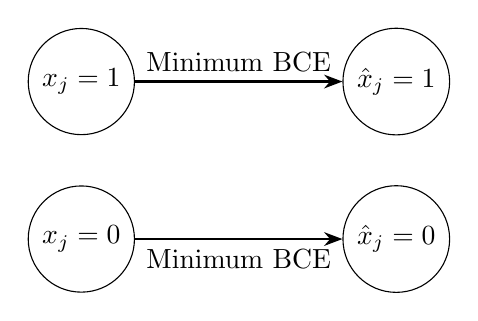
\begin{tikzpicture}[>=Stealth]
			
			\node[circle,draw] (x1) at (0,1) {$x_j=1$};
			\node[circle,draw] (y1) at (4,1) {$\hat{x}_j=1$};
			
			\node[circle,draw] (x0) at (0,-1) {$x_j=0$};
			\node[circle,draw] (y0) at (4,-1) {$\hat{x}_j=0$};
			
			\draw[->,thick] (x1)--(y1)
			node[midway,above]
			{Minimum BCE};
			
			\draw[->,thick] (x0)--(y0)
			node[midway,below]
			{Minimum BCE};
			
		\end{tikzpicture}
	\end{center}
	
	%%%%%%%%%%%%%%%%%%%%%%%%%%%%%%%%%%%%%%%%%%%%%%%%%%%%%%%%%%%%%%%%%%%%%%%%%%
	\section{Applications of Autoencoders}
	%%%%%%%%%%%%%%%%%%%%%%%%%%%%%%%%%%%%%%%%%%%%%%%%%%%%%%%%%%%%%%%%%%%%%%%%%%
	
	Autoencoders have become one of the most important unsupervised learning
	techniques because they can automatically learn useful representations of data.
	Some important applications are discussed below.
	
	%%%%%%%%%%%%%%%%%%%%%%%%%%%%%%%%%%%%%%%%%%%%%%%%%%%%%%%%%%%%%%%%%%%%%%%%%%
	\subsection{1. Dimensionality Reduction}
	%%%%%%%%%%%%%%%%%%%%%%%%%%%%%%%%%%%%%%%%%%%%%%%%%%%%%%%%%%%%%%%%%%%%%%%%%%
	
	The hidden layer of an undercomplete autoencoder learns a compact
	representation of the input data.
	
	Instead of storing the original high-dimensional input
	
	\[
	x\in\mathbb{R}^{n},
	\]
	
	the encoder produces
	
	\[
	h\in\mathbb{R}^{k},
	\qquad k<n.
	\]
	
	This lower-dimensional representation retains most of the useful information.
	
	Unlike Principal Component Analysis (PCA), an autoencoder can learn
	\textbf{non-linear} transformations.
	
%	\begin{center}
%		\begin{tikzpicture}[>=Stealth]
%			
%			\node[draw,minimum width=2.3cm,minimum height=1.3cm] (x) at (0,0){Input\\100 dims};
%			
%			\node[draw,minimum width=1.2cm,minimum height=1.0cm] (h) at (4,0){Code\\10 dims};
%			
%			\node[draw,minimum width=2.3cm,minimum height=1.3cm] (y) at (8,0){Reconstruction\\100 dims};
%			
%			\draw[->,thick](x)--node[above]{Encoder}(h);
%			\draw[->,thick](h)--node[above]{Decoder}(y);
%			
%		\end{tikzpicture}
%	\end{center}
%	
	%%%%%%%%%%%%%%%%%%%%%%%%%%%%%%%%%%%%%%%%%%%%%%%%%%%%%%%%%%%%%%%%%%%%%%%%%%
	\subsection{2. Image Denoising}
	%%%%%%%%%%%%%%%%%%%%%%%%%%%%%%%%%%%%%%%%%%%%%%%%%%%%%%%%%%%%%%%%%%%%%%%%%%
	
	Suppose the input image is corrupted by random noise,
	
	\[
	x=x_{\text{clean}}+\text{noise}.
	\]
	
	Instead of reconstructing the noisy image, the autoencoder is trained to
	produce the clean image.
	
	\[
	x_{\text{noisy}}
	\longrightarrow
	\text{Encoder}
	\longrightarrow
	h
	\longrightarrow
	\text{Decoder}
	\longrightarrow
	x_{\text{clean}}.
	\]
	
	The loss function becomes
	
	\[
	\boxed{
		L
		=
		\|x_{\text{clean}}
		-
		\hat{x}\|^2.
	}
	\]
	
	The network therefore learns to remove unwanted disturbances.
	
	%%%%%%%%%%%%%%%%%%%%%%%%%%%%%%%%%%%%%%%%%%%%%%%%%%%%%%%%%%%%%%%%%%%%%%%%%%
	\subsection{3. Anomaly Detection}
	%%%%%%%%%%%%%%%%%%%%%%%%%%%%%%%%%%%%%%%%%%%%%%%%%%%%%%%%%%%%%%%%%%%%%%%%%%
	
	An autoencoder is trained only on normal data.
	
	During testing,
	
	\[
	e
	=
	\|x-\hat{x}\|^2
	\]
	
	is computed.
	
	If
	
	\[
	e>\tau,
	\]
	
	where $\tau$ is a threshold,
	
	the sample is declared an anomaly.
	
	Examples include
	
	\begin{itemize}
		\item Credit card fraud detection
		\item Industrial fault detection
		\item Network intrusion detection
		\item Medical diagnosis
	\end{itemize}
	
	\begin{center}
		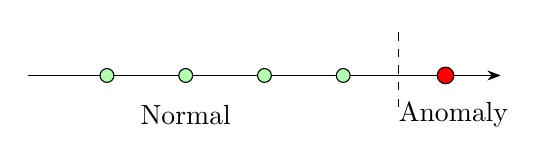
\begin{tikzpicture}[>=Stealth]
			
			\draw[->](0,0)--(6,0);
			
			\draw[fill=green!30] (1,0) circle (2.5pt);
			\draw[fill=green!30] (2,0) circle (2.5pt);
			\draw[fill=green!30] (3,0) circle (2.5pt);
			\draw[fill=green!30] (4,0) circle (2.5pt);
			
			\draw[fill=red] (5.3,0) circle (3pt);
			
			\draw[dashed](4.7,-0.4)--(4.7,0.6);
			
			\node at (2,-0.5){Normal};
			\node at (5.4,-0.5){Anomaly};
			
		\end{tikzpicture}
	\end{center}
	
	%%%%%%%%%%%%%%%%%%%%%%%%%%%%%%%%%%%%%%%%%%%%%%%%%%%%%%%%%%%%%%%%%%%%%%%%%%
	\subsection{4. Data Compression}
	%%%%%%%%%%%%%%%%%%%%%%%%%%%%%%%%%%%%%%%%%%%%%%%%%%%%%%%%%%%%%%%%%%%%%%%%%%
	
	Instead of storing the original data,
	
	\[
	x\in\mathbb{R}^{n},
	\]
	
	only the latent representation
	
	\[
	h\in\mathbb{R}^{k},
	\qquad k\ll n,
	\]
	
	is stored.
	
	Whenever needed,
	
	\[
	\hat{x}=f(h)
	\]
	
	is reconstructed.
	
	Compression ratio is
	
	\[
	\boxed{
		\text{Compression Ratio}
		=
		\frac{n}{k}.
	}
	\]
	
	%%%%%%%%%%%%%%%%%%%%%%%%%%%%%%%%%%%%%%%%%%%%%%%%%%%%%%%%%%%%%%%%%%%%%%%%%%
	\subsection{5. Feature Extraction}
	%%%%%%%%%%%%%%%%%%%%%%%%%%%%%%%%%%%%%%%%%%%%%%%%%%%%%%%%%%%%%%%%%%%%%%%%%%
	
	The encoder automatically extracts meaningful features.
	
	Instead of manually designing features,
	
	\[
	x
	\longrightarrow
	h,
	\]
	
	where
	
	\[
	h=
	g(Wx+b)
	\]
	
	contains the important characteristics of the input.
	
	These features can later be used for
	
	\begin{itemize}
		\item Classification
		\item Regression
		\item Clustering
		\item Visualization
	\end{itemize}
	
	%%%%%%%%%%%%%%%%%%%%%%%%%%%%%%%%%%%%%%%%%%%%%%%%%%%%%%%%%%%%%%%%%%%%%%%%%%
	\subsection{6. Recommendation Systems}
	%%%%%%%%%%%%%%%%%%%%%%%%%%%%%%%%%%%%%%%%%%%%%%%%%%%%%%%%%%%%%%%%%%%%%%%%%%
	
	Autoencoders are widely used in recommender systems.
	
	Suppose
	
	\[
	x=
	\begin{bmatrix}
		5\\
		4\\
		?\\
		1\\
		?
	\end{bmatrix}
	\]
	
	represents ratings given by a user.
	
	The encoder learns latent user preferences.
	
	The decoder predicts the missing entries.
	
	\[
	\hat{x}
	=
	\begin{bmatrix}
		5\\
		4\\
		3.8\\
		1\\
		4.6
	\end{bmatrix}
	\]
	
	Examples include
	
	\begin{itemize}
		\item Netflix
		\item Amazon
		\item YouTube
		\item Spotify
	\end{itemize}
	
	%%%%%%%%%%%%%%%%%%%%%%%%%%%%%%%%%%%%%%%%%%%%%%%%%%%%%%%%%%%%%%%%%%%%%%%%%%
	\subsection{7. Image and Video Applications}
	%%%%%%%%%%%%%%%%%%%%%%%%%%%%%%%%%%%%%%%%%%%%%%%%%%%%%%%%%%%%%%%%%%%%%%%%%%
	
	Autoencoders have numerous applications in computer vision.
	
	Some important applications include
	
	\begin{enumerate}
		\item Super-resolution
		\item Colorization
		\item Image Segmentation
		\item Face Recognition
		\item Pose Estimation
		\item Image Restoration
		\item Video Reconstruction
	\end{enumerate}
	
%	\begin{center}
%		\begin{tikzpicture}[>=Stealth]
%			
%			\node[draw,minimum width=2cm,minimum height=1.5cm](img) at (0,0){Image};
%			
%			\node[draw,minimum width=1.3cm,minimum height=1cm](enc) at (3,0){Encoder};
%			
%			\node[draw,minimum width=1.3cm,minimum height=1cm](code) at (6,0){Latent\\Features};
%			
%			\node[draw,minimum width=1.3cm,minimum height=1cm](dec) at (9,0){Decoder};
%			
%			\node[draw,minimum width=2cm,minimum height=1.5cm](out) at (12,0){Enhanced\\Image};
%			
%			\draw[->](img)--(enc);
%			\draw[->](enc)--(code);
%			\draw[->](code)--(dec);
%			\draw[->](dec)--(out);
%			
%		\end{tikzpicture}
%	\end{center}
%	
	%%%%%%%%%%%%%%%%%%%%%%%%%%%%%%%%%%%%%%%%%%%%%%%%%%%%%%%%%%%%%%%%%%%%%%%%%%
	\subsection{Summary of Applications}
	%%%%%%%%%%%%%%%%%%%%%%%%%%%%%%%%%%%%%%%%%%%%%%%%%%%%%%%%%%%%%%%%%%%%%%%%%%
	
	\begin{table}[H]
		\centering
		\caption{Major Applications of Autoencoders}
		\begin{tabular}{|c|p{8cm}|}
			\hline
			Application & Purpose\\
			\hline
			Dimensionality Reduction & Learn compact representations\\
			\hline
			Denoising & Remove unwanted noise from data\\
			\hline
			Anomaly Detection & Detect unusual samples\\
			\hline
			Compression & Reduce storage requirements\\
			\hline
			Feature Learning & Learn useful hidden representations\\
			\hline
			Recommendation Systems & Predict missing preferences\\
			\hline
			Computer Vision & Super-resolution, segmentation, face recognition, restoration\\
			\hline
		\end{tabular}
	\end{table}
	
	%%%%%%%%%%%%%%%%%%%%%%%%%%%%%%%%%%%%%%%%%%%%%%%%%%%%%%%%%%%%%%%%%%%%%%%%%%
	\section{Key Points}
	%%%%%%%%%%%%%%%%%%%%%%%%%%%%%%%%%%%%%%%%%%%%%%%%%%%%%%%%%%%%%%%%%%%%%%%%%%
	
	\begin{itemize}
		\item Autoencoders are unsupervised neural networks.
		
		\item They learn by reconstructing the input.
		
		\item The encoder compresses the information.
		
		\item The decoder reconstructs the original input.
		
		\item Undercomplete autoencoders perform dimensionality reduction.
		
		\item Overcomplete autoencoders require regularization.
		
		\item Binary Cross-Entropy is preferred for binary inputs.
		
		\item Mean Squared Error is preferred for continuous-valued inputs.
		
		\item Autoencoders form the basis of many modern deep learning models such as
		Variational Autoencoders (VAEs), Denoising Autoencoders, Sparse Autoencoders,
		Contractive Autoencoders, and Diffusion-based representation learning.
	\end{itemize}
	
%######### PCA and AE equivalence #########################
%%%%%%%%%%%%%%%%%%%%%%%%%%%%%%%%%%%%%%%%%%%%%%%%%%%%%%%%%%%%%%%%%%%%%%%%%%%%%%
\section{Link Between PCA and Autoencoder}
%%%%%%%%%%%%%%%%%%%%%%%%%%%%%%%%%%%%%%%%%%%%%%%%%%%%%%%%%%%%%%%%%%%%%%%%%%%%%%

We now establish the relationship between Principal Component Analysis (PCA)
and Autoencoders.

\begin{figure}[!ht]
	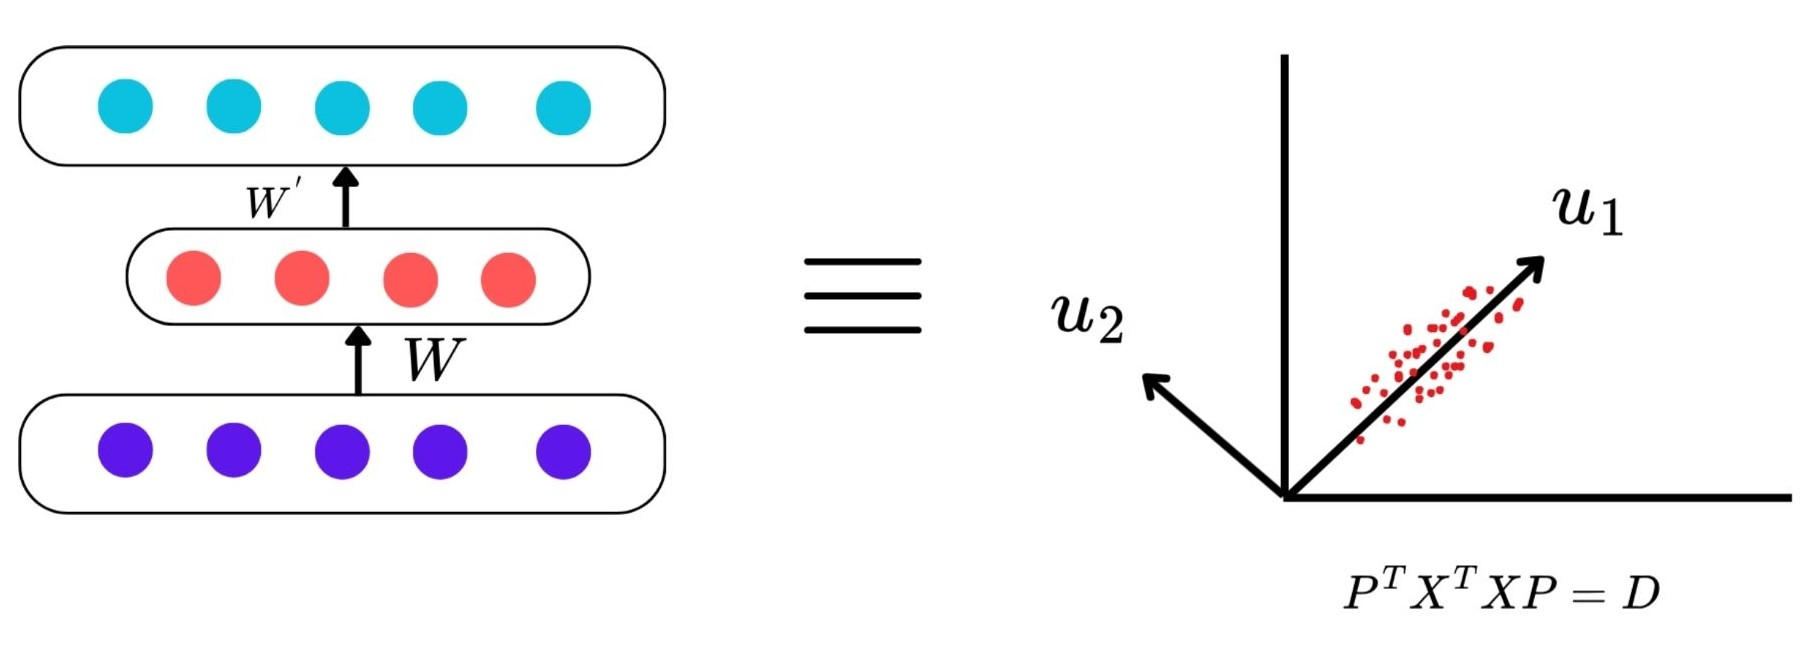
\includegraphics[width=0.8\linewidth]{images/AE_PCA.jpg}
\end{figure}

\begin{center}
	\begin{tikzpicture}[>=Stealth,scale=1]
		
		% Autoencoder
		\node[draw,ellipse,minimum width=2.5cm,minimum height=0.9cm] (x) at (0,0){};
		\foreach \i in {-0.6,0,0.6}
		\fill (\i,0) circle (2pt);
		
		\node[draw,ellipse,minimum width=1.6cm,minimum height=0.8cm] (h) at (0,2){};
		\foreach \i in {-0.25,0.25}
		\fill (\i,2) circle (2pt);
		
		\node[draw,ellipse,minimum width=2.5cm,minimum height=0.9cm] (y) at (0,4){};
		\foreach \i in {-0.6,0,0.6}
		\fill (\i,4) circle (2pt);
		
		\draw[->,thick](x)--(h);
		\draw[->,thick](h)--(y);
		
		% PCA axes
		\draw[->] (5,-0.2)--(5,3);
		\draw[->] (5,-0.2)--(8,-0.2);
		
		\draw[->,thick] (5,-0.2)--(6.9,2.2);
		\draw[->,thick] (5,-0.2)--(4.2,1.4);
		
		\node at (7.2,2.3){$u_1$};
		\node at (4.0,1.5){$u_2$};
		
		\node at (6.2,-0.9)
		{$P^{T}X^{T}XP=D$};
		
	\end{tikzpicture}
\end{center}

We shall now show that the encoder part of an Autoencoder is equivalent to
Principal Component Analysis provided the following conditions are satisfied.

\begin{enumerate}
	\item A \textbf{linear encoder} is used.
	\item A \textbf{linear decoder} is used.
	\item The reconstruction loss is the squared error loss.
	\item The input data are normalized (zero mean).
\end{enumerate}

%%%%%%%%%%%%%%%%%%%%%%%%%%%%%%%%%%%%%%%%%%%%%%%%%%%%%%%%%%%%%%%%%%%%%%%%%%%%%%
\subsection{Normalization of the Input Data}
%%%%%%%%%%%%%%%%%%%%%%%%%%%%%%%%%%%%%%%%%%%%%%%%%%%%%%%%%%%%%%%%%%%%%%%%%%%%%%

Each feature is normalized according to

\[
\boxed{
	\hat{x}_{ij}
	=
	\frac{1}{\sqrt{m}}
	\left(
	x_{ij}
	-
	\frac1m
	\sum_{k=1}^{m}x_{kj}
	\right)
}
\]

where

\[
\mu_j
=
\frac1m
\sum_{k=1}^{m}x_{kj}
\]

is the mean of the $j^{th}$ feature.

The quantity inside the brackets subtracts the feature mean from every sample.
Hence, after normalization,

\[
\boxed{
	\sum_{i=1}^{m}\hat{x}_{ij}=0,
	\qquad
	j=1,\ldots,n.
}
\]

Therefore, every feature has zero mean.

Let

\[
X'
\]

denote the zero-mean data matrix.

Then,

\[
\boxed{
	\hat{X}
	=
	\frac1{\sqrt m}X'.
}
\]

Consequently,

\[
\begin{aligned}
	\hat{X}^{T}\hat{X}
	&=
	\left(\frac1{\sqrt m}X'\right)^T
	\left(\frac1{\sqrt m}X'\right)\\
	&=
	\frac1m(X')^TX'.
\end{aligned}
\]

Since

\[
\boxed{
	C=\frac1m(X')^TX',
}
\]

we obtain

\[
\boxed{
	\hat{X}^{T}\hat{X}=C,
}
\]

which is exactly the covariance matrix used in PCA.

%%%%%%%%%%%%%%%%%%%%%%%%%%%%%%%%%%%%%%%%%%%%%%%%%%%%%%%%%%%%%%%%%%%%%%%%%%%%%%
\subsection{Linear Autoencoder Objective}
%%%%%%%%%%%%%%%%%%%%%%%%%%%%%%%%%%%%%%%%%%%%%%%%%%%%%%%%%%%%%%%%%%%%%%%%%%%%%%

Assume that both encoder and decoder are linear.

The reconstruction loss is

\[
\boxed{
	J
	=
	\frac1m
	\sum_{i=1}^{m}
	\sum_{j=1}^{n}
	\left(
	x_{ij}
	-
	\hat{x}_{ij}
	\right)^2.
}
\]

Equivalently,

\[
\boxed{
	\min_{\theta}
	\sum_{i=1}^{m}
	\sum_{j=1}^{n}
	(x_{ij}-\hat{x}_{ij})^2.
}
\]

Since

\[
\hat{X}=HW^{T},
\]

the optimization problem can be written compactly as

\[
\boxed{
	\min_{H,W}
	\|
	X-HW^{T}
	\|_{F}^{2},
}
\]

where

\[
\|A\|_{F}
=
\sqrt{
	\sum_{i=1}^{m}
	\sum_{j=1}^{n}
	a_{ij}^{2}
}
\]

is the Frobenius norm.

The matrices involved are

\[
X
=
\begin{bmatrix}
	x_1\\
	x_2\\
	\vdots\\
	x_m
\end{bmatrix}
\in\mathbb{R}^{m\times n},
\]

\[
H
=
\begin{bmatrix}
	h_1\\
	h_2\\
	\vdots\\
	h_m
\end{bmatrix}
\in\mathbb{R}^{m\times k},
\]

and

\[
W
\in
\mathbb{R}^{n\times k}.
\]

Hence,

\[
\boxed{
	\hat{X}=HW^{T}.
}
\]

%%%%%%%%%%%%%%%%%%%%%%%%%%%%%%%%%%%%%%%%%%%%%%%%%%%%%%%%%%%%%%%%%%%%%%%%%%%%%%
\subsection{Optimal Solution using Singular Value Decomposition (SVD)}
%%%%%%%%%%%%%%%%%%%%%%%%%%%%%%%%%%%%%%%%%%%%%%%%%%%%%%%%%%%%%%%%%%%%%%%%%%%%%%

The optimization problem obtained previously is

\[
\boxed{
	\min_{H,W}
	\left\|
	X-HW^{T}
	\right\|_{F}^{2}.
}
\tag{1}
\]

Recall the Singular Value Decomposition (SVD) of the data matrix,

\[
\boxed{
	X=U\Sigma V^{T}.
}
\]

From the Eckart--Young theorem, the best rank-$k$ approximation of $X$ is

\[
\boxed{
	X_k
	=
	U_{(:,1:k)}
	\Sigma_{1:k,1:k}
	V_{(:,1:k)}^{T}.
}
\]

Therefore, the optimal reconstruction satisfying (1) is

\[
\boxed{
	HW^{T}
	=
	U_{(:,1:k)}
	\Sigma_{1:k,1:k}
	V_{(:,1:k)}^{T}.
}
\]

One possible choice satisfying this equality is

\[
\boxed{
	H
	=
	U_{(:,1:k)}
	\Sigma_{1:k,1:k},
}
\]

and

\[
\boxed{
	W
	=
	V_{(:,1:k)}.
}
\]

Thus,

\[
HW^{T}
=
U_{(:,1:k)}
\Sigma_{1:k,1:k}
V_{(:,1:k)}^{T}.
\]

Hence the linear decoder weights correspond to the first $k$ right singular
vectors of the data matrix.

%%%%%%%%%%%%%%%%%%%%%%%%%%%%%%%%%%%%%%%%%%%%%%%%%%%%%%%%%%%%%%%%%%%%%%%%%%%%%%
\subsection{Derivation of the Encoder Matrix}
%%%%%%%%%%%%%%%%%%%%%%%%%%%%%%%%%%%%%%%%%%%%%%%%%%%%%%%%%%%%%%%%%%%%%%%%%%%%%%

We now derive the encoder representation.

Recall that

\[
H=XW.
\]

Substituting the optimal decoder,

\[
W
=
V_{(:,1:k)},
\]

gives

\[
H
=
XV_{(:,1:k)}.
\]

To verify this using the SVD expansion,

\[
X
=
U\Sigma V^{T},
\]

we write

\[
\begin{aligned}
	H
	&=
	XV_{(:,1:k)}
	\\
	&=
	U\Sigma V^{T}V_{(:,1:k)}.
\end{aligned}
\]

Since

\[
V^{T}V=I,
\]

we obtain

\[
\boxed{
	H
	=
	U\Sigma_{(:,1:k)}.
}
\]

This is exactly the expression obtained from the optimal rank-$k$
approximation.

%%%%%%%%%%%%%%%%%%%%%%%%%%%%%%%%%%%%%%%%%%%%%%%%%%%%%%%%%%%%%%%%%%%%%%%%%%%%%%
\subsection{Alternative Proof Using the Moore--Penrose Inverse}
%%%%%%%%%%%%%%%%%%%%%%%%%%%%%%%%%%%%%%%%%%%%%%%%%%%%%%%%%%%%%%%%%%%%%%%%%%%%%%

Previously, we obtained

\[
H^{*}=U_{(:,1:k)}\Sigma_{(1:k,1:k)}.
\]

The encoder weight matrix is

\[
W^{*}=X^{+}H^{*},
\]

where \(X^{+}\) denotes the Moore--Penrose pseudoinverse.

Using

\[
X^{+}
=
(X^{T}X)^{-1}X^{T},
\]

we obtain

\[
W^{*}
=
(X^{T}X)^{-1}
X^{T}
U_{(:,1:k)}
\Sigma_{(1:k,1:k)}.
\]

Now substitute the Singular Value Decomposition

\[
X=U\Sigma V^{T}.
\]

Hence,

\[
=
\left(
V\Sigma^{T}U^{T}
U\Sigma V^{T}
\right)^{-1}
\left(
V\Sigma^{T}U^{T}
\right)
U_{(:,1:k)}
\Sigma_{(1:k,1:k)}.
\]

\hfill (using \(X=U\Sigma V^{T}\))

Since

\[
U^{T}U=I,
\]

the above becomes

\[
=
\left(
V\Sigma^{T}\Sigma V^{T}
\right)^{-1}
V\Sigma^{T}
U^{T}
U_{(:,1:k)}
\Sigma_{(1:k,1:k)}.
\]

Using

\[
(ABC)^{-1}
=
C^{-1}B^{-1}A^{-1},
\]

we obtain

\[
=
V
(\Sigma^{T}\Sigma)^{-1}
V^{T}
V
\Sigma^{T}
U^{T}
U_{(:,1:k)}
\Sigma_{(1:k,1:k)}.
\]

Since

\[
V^{T}V=I,
\]

this simplifies to

\[
=
V
(\Sigma^{T}\Sigma)^{-1}
\Sigma^{T}
U^{T}
U_{(:,1:k)}
\Sigma_{(1:k,1:k)}.
\]

Now observe that

\[
(\Sigma^{T}\Sigma)^{-1}\Sigma^{T}
=
\Sigma^{-1},
\]

therefore,

\[
=
V
\Sigma^{-1}
U^{T}
U_{(:,1:k)}
\Sigma_{(1:k,1:k)}.
\]

Since

\[
U^{T}U_{(:,1:k)}
=
I_{(:,1:k)},
\]

we obtain

\[
=
V
\Sigma^{-1}
I_{(:,1:k)}
\Sigma_{(1:k,1:k)}.
\]

Finally,

\[
\Sigma^{-1}
I_{(:,1:k)}
\Sigma_{(1:k,1:k)}
=
I_{(:,1:k)},
\]

which gives

\[
\boxed{
	W^{*}
	=
	V_{(:,1:k)}
}
\]

Hence, we have shown that the optimal encoder of a linear
autoencoder is

\[
\boxed{
	H=XW^{*}
	=
	XV_{(:,1:k)}.
}
\]

Therefore, the encoder performs a linear transformation using the first
\(k\) right singular vectors of \(X\).

Since the right singular vectors of \(X\) are precisely the eigenvectors
of \(X^{T}X\), the encoder weight matrix is identical to the projection
matrix used in Principal Component Analysis (PCA).

Thus,

\[
\boxed{
	W^{*}=P=V_{(:,1:k)}.
}
\]

Hence, the encoder of a linear autoencoder and the PCA projection matrix
are exactly the same.
%%%%%%%%%%%%%%%%%%%%%%%%%%%%%%%%%%%%%%%%%%%%%%%%%%%%%%%%%%%%%%%%%%%%%%%%%%%%%%
\subsection{Connection with PCA}
%%%%%%%%%%%%%%%%%%%%%%%%%%%%%%%%%%%%%%%%%%%%%%%%%%%%%%%%%%%%%%%%%%%%%%%%%%%%%%

From Singular Value Decomposition,

\[
\boxed{
	W
	=
	V_{(:,1:k)}.
}
\]

From PCA, the projection matrix is formed by the eigenvectors of the covariance
matrix

\[
C
=
\frac{1}{m}X^{T}X.
\]

Since

\[
X^{T}X
=
V\Sigma^{2}V^{T},
\]

the columns of $V$ are precisely the eigenvectors of the covariance matrix.

Therefore,

\[
\boxed{
	P
	=
	V_{(:,1:k)}.
}
\]

Consequently,

\[
\boxed{
	W=P.
}
\]

That is, the encoder matrix learned by a linear autoencoder is exactly the PCA
projection matrix.

%%%%%%%%%%%%%%%%%%%%%%%%%%%%%%%%%%%%%%%%%%%%%%%%%%%%%%%%%%%%%%%%%%%%%%%%%%%%%%
\subsection{Final Result}
%%%%%%%%%%%%%%%%%%%%%%%%%%%%%%%%%%%%%%%%%%%%%%%%%%%%%%%%%%%%%%%%%%%%%%%%%%%%%%

We have shown that the encoder of a linear autoencoder is equivalent to PCA
provided the following conditions are satisfied.

\begin{enumerate}
	\item A linear encoder is used.
	\item A linear decoder is used.
	\item The reconstruction loss is the squared-error loss.
	\item The input data are normalized to have zero mean.
\end{enumerate}

Since the normalized data satisfy

\[
\boxed{
	\hat{x}_{ij}
	=
	\frac{1}{\sqrt{m}}
	\left(
	x_{ij}
	-
	\frac1m
	\sum_{k=1}^{m}
	x_{kj}
	\right),
}
\]

the covariance matrix becomes

\[
\boxed{
	C
	=
	\hat{X}^{T}\hat{X},
}
\]

whose eigenvectors are exactly

\[
\boxed{
	V.
}
\]

Hence,

\[
\boxed{
	\text{Linear Autoencoder Encoder}
	=
	\text{PCA Projection Matrix}.
}
\]

%%%%%%%%%%%%%%%%%%%%%%%%%%%%%%%%%%%%%%%%%%%%%%%%%%%%%%%%%%%%%%%%%%%%%%%%%%%%%%
\begin{tcolorbox}[title=Important Result,colback=blue!5,colframe=blue!60]
	
	The encoder of a linear autoencoder is equivalent to Principal Component
	Analysis (PCA) if
	
	\begin{itemize}
		\item the encoder is linear,
		\item the decoder is linear,
		\item the reconstruction loss is Mean Squared Error,
		\item and the input data are centered (zero mean).
	\end{itemize}
	
	Under these assumptions,
	
	\[
	\boxed{
		W=P=V_{(:,1:k)},
	}
	\]
	
	where $V_{(:,1:k)}$ contains the first $k$ eigenvectors (principal components)
	of the covariance matrix.
	
\end{tcolorbox}

%%%%%%%%%%%%%%%%%%%%%%%%%%%%%%%%%%%%%%%%%%%%%%%%%%%%%%%%%%%%%%
\section{Equivalence of Linear Autoencoder and PCA (Continued)}
%%%%%%%%%%%%%%%%%%%%%%%%%%%%%%%%%%%%%%%%%%%%%%%%%%%%%%%%%%%%%%

From the previous derivation, we obtained

\[
W = V_{(:,1:k)},
\]

where \(V_{(:,1:k)}\) denotes the first \(k\) eigenvectors (principal
components) of the covariance matrix.

Recall that the normalized data matrix is

\[
\hat{x}_{ij}
=
\frac{1}{\sqrt{m}}
\left(
x_{ij}
-
\frac{1}{m}
\sum_{l=1}^{m}x_{lj}
\right),
\]

which centers every feature so that its mean becomes zero.

Since

\[
X=\frac{1}{\sqrt{m}}X',
\]

the covariance matrix becomes

\[
X^{T}X
=
\frac{1}{m}(X')^{T}X'.
\]

The covariance matrix plays the central role in Principal Component
Analysis.

Since

\[
X=U\Sigma V^{T},
\]

the eigenvectors of

\[
X^{T}X
\]

are exactly the columns of

\[
V.
\]

Therefore,

\[
W=V_{(:,1:k)}
\]

is precisely the PCA projection matrix.

Hence, the encoder of a linear autoencoder performs the same projection
as Principal Component Analysis.

%%%%%%%%%%%%%%%%%%%%%%%%%%%%%%%%%%%%%%%%%%%%%%%%%%%%%%%%%%%%%%
\subsection{Important Result}
%%%%%%%%%%%%%%%%%%%%%%%%%%%%%%%%%%%%%%%%%%%%%%%%%%%%%%%%%%%%%%

The encoder of a linear autoencoder is equivalent to PCA provided that

\begin{enumerate}
	\item the encoder is linear,
	\item the decoder is linear,
	\item the reconstruction loss is Mean Squared Error,
	\item the input data are centered (zero mean).
\end{enumerate}

Under these assumptions,

\[
\boxed{
	W=P=V_{(:,1:k)}
}
\]

where \(P\) is the PCA projection matrix.

%%%%%%%%%%%%%%%%%%%%%%%%%%%%%%%%%%%%%%%%%%%%%%%%%%%%%%%%%%%%%%
\section{Relationship Between PCA and Autoencoder}
%%%%%%%%%%%%%%%%%%%%%%%%%%%%%%%%%%%%%%%%%%%%%%%%%%%%%%%%%%%%%%

Figure~\ref{fig:pca_autoencoder} illustrates the similarity between a
linear autoencoder and Principal Component Analysis.

\begin{figure}[H]
	\centering
	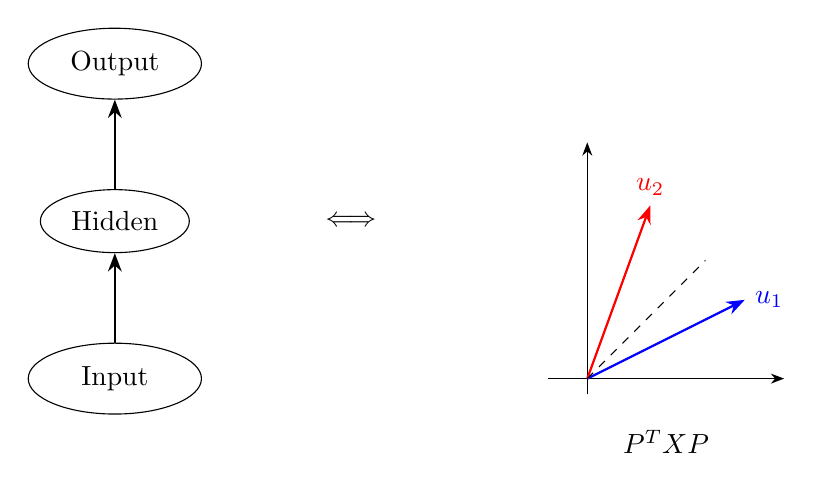
\begin{tikzpicture}[>=Stealth,scale=1]
		
		%---------------- Autoencoder ----------------%
		
		\node[draw,ellipse,minimum width=2.2cm,minimum height=0.9cm] (in) at (0,0)
		{Input};
		
		\node[draw,ellipse,minimum width=1.6cm,minimum height=0.8cm] (hid) at (0,2)
		{Hidden};
		
		\node[draw,ellipse,minimum width=2.2cm,minimum height=0.9cm] (out) at (0,4)
		{Output};
		
		\draw[->,thick] (in)--(hid);
		\draw[->,thick] (hid)--(out);
		
		\node at (3,2){$\Longleftrightarrow$};
		
		%---------------- PCA ----------------%
		
		\draw[->] (6,-0.2)--(6,3);
		\draw[->] (5.5,0)--(8.5,0);
		
		\draw[thick,blue,->] (6,0)--(8,1)
		node[right]{$u_1$};
		
		\draw[thick,red,->] (6,0)--(6.8,2.2)
		node[above]{$u_2$};
		
		\draw[dashed] (6,0)--(7.5,1.5);
		
		\node at (7,-0.8)
		{$P^{T}XP$};
		
	\end{tikzpicture}
	
	\caption{Connection between Linear Autoencoder and PCA}
	\label{fig:pca_autoencoder}
\end{figure}

%%%%%%%%%%%%%%%%%%%%%%%%%%%%%%%%%%%%%%%%%%%%%%%%%%%%%%%%%%%%%%
\section{Summary}
%%%%%%%%%%%%%%%%%%%%%%%%%%%%%%%%%%%%%%%%%%%%%%%%%%%%%%%%%%%%%%

For a linear autoencoder,

\[
H=XW,
\]

where

\[
W=V_{(:,1:k)}.
\]

The reconstruction is

\[
\hat{X}=HW^{T}.
\]

Therefore,

\[
\hat{X}
=
XV_{(:,1:k)}
V_{(:,1:k)}^{T},
\]

which is exactly the rank-\(k\) approximation obtained from Principal
Component Analysis.

Hence,

\[
\boxed{
	\text{Linear Autoencoder}
	\equiv
	\text{PCA}
}
\]

when

\begin{itemize}
	\item encoder is linear,
	\item decoder is linear,
	\item reconstruction loss is MSE,
	\item inputs are centered.
\end{itemize}

%%%%%%%%%%%%%%%%%%%%%%%%%%%%%%%%%%%%%%%%%%%%%%%%%%%%%%%%%%%%%%
\section{Advantages of Autoencoders over PCA}
%%%%%%%%%%%%%%%%%%%%%%%%%%%%%%%%%%%%%%%%%%%%%%%%%%%%%%%%%%%%%%

Although linear autoencoders reduce to PCA, practical autoencoders are
generally nonlinear.

Their major advantages are

\begin{itemize}
	\item Nonlinear feature extraction.
	\item Deep hierarchical representations.
	\item Better reconstruction for complex data.
	\item Ability to model images, speech and text.
	\item Easy integration with CNNs, RNNs and Transformers.
	\item Can be trained using gradient descent.
\end{itemize}

Thus,

\[
\boxed{
	\text{PCA is a special case of a Linear Autoencoder.}
}
\]

A nonlinear autoencoder extends PCA by replacing the linear encoder and
decoder with nonlinear neural networks.

%%%%%%%%%%%%%%%%%%%%%%%%%%%%%%%%%%%%%%%%%%%%%%%%%%%%%%%%%%%%%%
\section{Transition to Deep Autoencoders}
%%%%%%%%%%%%%%%%%%%%%%%%%%%%%%%%%%%%%%%%%%%%%%%%%%%%%%%%%%%%%%

Instead of

\[
h=f(Wx+b),
\]

we may use multiple hidden layers:

\[
x
\rightarrow
h_1
\rightarrow
h_2
\rightarrow
\cdots
\rightarrow
h_k
\rightarrow
\hat{x}.
\]

This leads to Deep Autoencoders, which can learn highly nonlinear latent
representations that are impossible to obtain using classical PCA.

%============== Denoising Auto Encoers ========================
%%%%%%%%%%%%%%%%%%%%%%%%%%%%%%%%%%%%%%%%%%%%%%%%%%%%%%%%%%%%%%
\section{Denoising Autoencoder}
%%%%%%%%%%%%%%%%%%%%%%%%%%%%%%%%%%%%%%%%%%%%%%%%%%%%%%%%%%%%%%

A denoising autoencoder is a special type of autoencoder in which the
input data is deliberately corrupted before being given to the
network. The objective of the network is to reconstruct the original
uncorrupted input.

The basic idea is

\[
\boxed{
	\text{Corrupted Input}
	\longrightarrow
	\text{Encoder}
	\longrightarrow
	\text{Decoder}
	\longrightarrow
	\text{Reconstructed Input}
}
\]

The important difference from a conventional autoencoder is that the
network receives a corrupted version of the input but is trained to
reconstruct the original input.

%%%%%%%%%%%%%%%%%%%%%%%%%%%%%%%%%%%%%%%%%%%%%%%%%%%%%%%%%%%%%%
\subsection{Basic Architecture}
%%%%%%%%%%%%%%%%%%%%%%%%%%%%%%%%%%%%%%%%%%%%%%%%%%%%%%%%%%%%%%

Let the original input be

\[
x_i \in \mathbb{R}^{n}.
\]

A corrupted version of the input is denoted by

\[
\widetilde{x}_i.
\]

The corruption process is represented by

\[
\widetilde{x}_i
\sim
P(\widetilde{x}_i\mid x_i).
\]

The corrupted input is then passed through the encoder:

\[
h_i
=
g(W\widetilde{x}_i+b).
\]

The decoder reconstructs the original input:

\[
\widehat{x}_i
=
f(W'h_i+c).
\]

Therefore,

\[
\boxed{
	x_i
	\longrightarrow
	\widetilde{x}_i
	\longrightarrow
	h_i
	\longrightarrow
	\widehat{x}_i
}
\]

where

\begin{itemize}
	\item \(x_i\) is the original input,
	\item \(\widetilde{x}_i\) is the corrupted input,
	\item \(h_i\) is the hidden representation,
	\item \(\widehat{x}_i\) is the reconstructed output.
\end{itemize}


%%%%%%%%%%%%%%%%%%%%%%%%%%%%%%%%%%%%%%%%%%%%%%%%%%%%%%%%%%%%%%
\subsection{Denoising Autoencoder Architecture}
%%%%%%%%%%%%%%%%%%%%%%%%%%%%%%%%%%%%%%%%%%%%%%%%%%%%%%%%%%%%%%

The architecture can be represented as follows.

\begin{figure}[H]
	\centering
	
	\begin{tikzpicture}[
		>=Stealth,
		node distance=1.7cm,
		neuron/.style={
			draw,
			circle,
			minimum size=0.75cm,
			inner sep=0pt
		},
		layer/.style={
			draw,
			rounded corners=8pt,
			minimum width=2.7cm,
			minimum height=1.2cm
		},
		every node/.style={font=\small}
		]
		
		% Input layer
		\node[layer] (input) {
			\begin{tikzpicture}
				\node[neuron] at (0,0) {};
				\node[neuron] at (0.65,0) {};
				\node[neuron] at (1.3,0) {};
			\end{tikzpicture}
		};
		
		% Corrupted layer
		\node[layer, right=1.7cm of input] (corrupt) {
			\begin{tikzpicture}
				\node[neuron] at (0,0) {};
				\node[neuron] at (0.65,0) {};
				\node[neuron] at (1.3,0) {};
			\end{tikzpicture}
		};
		
		% Hidden layer
		\node[layer, right=1.7cm of corrupt] (hidden) {
			\begin{tikzpicture}
				\node[neuron] at (0,0) {};
				\node[neuron] at (0.65,0) {};
			\end{tikzpicture}
		};
		
		% Output layer
		\node[layer, right=1.7cm of hidden] (output) {
			\begin{tikzpicture}
				\node[neuron] at (0,0) {};
				\node[neuron] at (0.65,0) {};
				\node[neuron] at (1.3,0) {};
			\end{tikzpicture}
		};
		
		% Labels
		\node[below=0.25cm of input] {$x_i$};
		\node[below=0.25cm of corrupt] {$\widetilde{x}_i$};
		\node[below=0.25cm of hidden] {$h_i$};
		\node[below=0.25cm of output] {$\widehat{x}_i$};
		
		% Arrows
		\draw[->,thick]
		(input) -- node[above] {corruption} (corrupt);
		
		\draw[->,thick]
		(corrupt) -- node[above] {$W,b$} (hidden);
		
		\draw[->,thick]
		(hidden) -- node[above] {$W',c$} (output);
		
		% Corruption probability
		\node[above=0.7cm of corrupt]
		{
			$\widetilde{x}_i
			\sim P(\widetilde{x}_i\mid x_i)$
		};
		
		% Encoder / decoder labels
		\node[above=0.65cm of hidden]
		{
			Encoder
		};
		
		\node[above=0.65cm of output]
		{
			Decoder
		};
		
	\end{tikzpicture}
	
	\caption{Architecture of a Denoising Autoencoder}
	\label{fig:denoising_autoencoder}
\end{figure}


%%%%%%%%%%%%%%%%%%%%%%%%%%%%%%%%%%%%%%%%%%%%%%%%%%%%%%%%%%%%%%
\subsection{Corruption Process}
%%%%%%%%%%%%%%%%%%%%%%%%%%%%%%%%%%%%%%%%%%%%%%%%%%%%%%%%%%%%%%

Consider an input vector

\[
x_i=
\begin{bmatrix}
	x_{i1} & x_{i2} & \cdots & x_{in}
\end{bmatrix}^{T}.
\]

A corrupted version of the input is generated using a corruption
distribution

\[
\boxed{
	P(\widetilde{x}_i\mid x_i)
}
\]

The corruption process changes some components of \(x_i\).

For example,

\[
x_i=
\begin{bmatrix}
	1&1&1&1&1
\end{bmatrix}
\]

may be transformed into

\[
\widetilde{x}_i=
\begin{bmatrix}
	1&0&1&0&1
\end{bmatrix}.
\]

Thus, some of the original features are intentionally removed or
corrupted.

%%%%%%%%%%%%%%%%%%%%%%%%%%%%%%%%%%%%%%%%%%%%%%%%%%%%%%%%%%%%%%
\subsection{Simple Corruption Model}
%%%%%%%%%%%%%%%%%%%%%%%%%%%%%%%%%%%%%%%%%%%%%%%%%%%%%%%%%%%%%%

A simple corruption process is obtained by randomly setting an input
feature to zero.

For each input component,

\[
x_{ij}\in\{0,1\},
\]

we can define

\[
P(\widetilde{x}_{ij}=0\mid x_{ij})
=q,
\]

and

\[
P(\widetilde{x}_{ij}=x_{ij}\mid x_{ij})
=1-q.
\]

Here,

\[
q
\]

is the probability of corrupting an input component.

Thus, with probability \(q\), an input feature is corrupted, while with
probability \(1-q\), it is retained.

For example, consider

\[
x_i=
\begin{bmatrix}
	1&1&1&1&1
\end{bmatrix}.
\]

After applying the corruption process, we may obtain

\[
\widetilde{x}_i=
\begin{bmatrix}
	1&0&0&1&1
\end{bmatrix}.
\]

The network receives

\[
\widetilde{x}_i
\]

but the desired output remains

\[
x_i.
\]

Therefore,

\[
\boxed{
	\widetilde{x}_i
	\neq
	x_i
}
\]

but

\[
\boxed{
	\widehat{x}_i
	\approx
	x_i.
}
\]


%%%%%%%%%%%%%%%%%%%%%%%%%%%%%%%%%%%%%%%%%%%%%%%%%%%%%%%%%%%%%%
\subsection{Encoder and Decoder}
%%%%%%%%%%%%%%%%%%%%%%%%%%%%%%%%%%%%%%%%%%%%%%%%%%%%%%%%%%%%%%

The corrupted input is passed through the encoder:

\[
\boxed{
	h_i=g(W\widetilde{x}_i+b)
}
\]

where

\[
W\in\mathbb{R}^{d\times n}.
\]

The hidden representation is then passed through the decoder:

\[
\boxed{
	\widehat{x}_i
	=
	f(W'h_i+c)
}
\]

where

\[
W'\in\mathbb{R}^{n\times d}.
\]

Combining both operations gives

\[
\widehat{x}_i
=
f\left(
W'g(W\widetilde{x}_i+b)+c
\right).
\]

The important point is that the decoder is not asked to reproduce the
corrupted input. Instead, it is trained to reproduce the original
input:

\[
\boxed{
	\widetilde{x}_i
	\longrightarrow
	\widehat{x}_i
	\approx
	x_i.
}
\]


%%%%%%%%%%%%%%%%%%%%%%%%%%%%%%%%%%%%%%%%%%%%%%%%%%%%%%%%%%%%%%
\subsection{Why Denoising Autoencoder?}
%%%%%%%%%%%%%%%%%%%%%%%%%%%%%%%%%%%%%%%%%%%%%%%%%%%%%%%%%%%%%%

In a conventional autoencoder, the network receives

\[
x_i
\]

and attempts to reconstruct

\[
x_i.
\]

Thus,

\[
x_i
\longrightarrow
h_i
\longrightarrow
\widehat{x}_i
\approx x_i.
\]

In a denoising autoencoder, the input is first corrupted:

\[
x_i
\longrightarrow
\widetilde{x}_i
\longrightarrow
h_i
\longrightarrow
\widehat{x}_i.
\]

However, the target remains the original input:

\[
\boxed{
	\widehat{x}_i
	\approx
	x_i.
}
\]

Therefore, the network is forced to learn the important underlying
features of the data rather than simply copying the input.

%%%%%%%%%%%%%%%%%%%%%%%%%%%%%%%%%%%%%%%%%%%%%%%%%%%%%%%%%%%%%%
\subsection{Reconstruction Objective}
%%%%%%%%%%%%%%%%%%%%%%%%%%%%%%%%%%%%%%%%%%%%%%%%%%%%%%%%%%%%%%

The objective of the denoising autoencoder is to minimize the
reconstruction error between the original input \(x_i\) and the
reconstructed output \(\widehat{x}_i\).

For \(m\) training examples, the Mean Squared Error objective is

\[
\boxed{
	\min_{\theta}
	\frac{1}{m}
	\sum_{i=1}^{m}
	\left\|
	x_i-\widehat{x}_i
	\right\|_2^2
}
\]

where

\[
\theta=\{W,b,W',c\}.
\]

Since

\[
\widehat{x}_i
=
f\left(
W'g(W\widetilde{x}_i+b)+c
\right),
\]

the complete objective becomes

\[
\boxed{
	\min_{W,W',b,c}
	\frac{1}{m}
	\sum_{i=1}^{m}
	\left\|
	x_i-
	f\left(
	W'g(W\widetilde{x}_i+b)+c
	\right)
	\right\|_2^2
}
\]

with

\[
\widetilde{x}_i
\sim
P(\widetilde{x}_i\mid x_i).
\]


%%%%%%%%%%%%%%%%%%%%%%%%%%%%%%%%%%%%%%%%%%%%%%%%%%%%%%%%%%%%%%
\subsection{Key Idea}
%%%%%%%%%%%%%%%%%%%%%%%%%%%%%%%%%%%%%%%%%%%%%%%%%%%%%%%%%%%%%%

The key idea behind a denoising autoencoder is therefore

\[
\boxed{
	\text{Corrupt the input}
	\quad\rightarrow\quad
	\text{encode the corrupted input}
	\quad\rightarrow\quad
	\text{reconstruct the original input}.
}
\]

The corruption process prevents the network from simply learning the
identity function.

Instead, the network must learn robust features that allow it to
recover the original data from a partially corrupted observation.

Thus,

\[
\boxed{
	\text{DAE learns robust representations by reconstructing clean data
		from corrupted data.}
}
\]

%%%%%%%%%%%%%%%%%%%%%%%%%%%%%%%%%%%%%%%%%%%%%%%%%%%%%%%%%%%%%%
\subsection{Effect of Corruption}
%%%%%%%%%%%%%%%%%%%%%%%%%%%%%%%%%%%%%%%%%%%%%%%%%%%%%%%%%%%%%%

Suppose the original input is

\[
x_i=
\begin{bmatrix}
	1&1&1&1&1
\end{bmatrix}^{T}.
\]

After corruption,

\[
\widetilde{x}_i=
\begin{bmatrix}
	1&0&0&1&1
\end{bmatrix}^{T}.
\]

The encoder receives

\[
h_i=g(W\widetilde{x}_i+b),
\]

and the decoder produces

\[
\widehat{x}_i
=
f(W'h_i+c).
\]

The target is still

\[
x_i=
\begin{bmatrix}
	1&1&1&1&1
\end{bmatrix}^{T}.
\]

Therefore, the training objective forces

\[
\widehat{x}_i
\rightarrow
x_i
\]

even though the network only receives

\[
\widetilde{x}_i.
\]

This makes the learned representation more robust to noise and missing
features.


%%%%%%%%%%%%%%%%%%%%%%%%%%%%%%%%%%%%%%%%%%%%%%%%%%%%%%%%%%%%%%
\subsection{Graphical Interpretation of the Corruption Process}
%%%%%%%%%%%%%%%%%%%%%%%%%%%%%%%%%%%%%%%%%%%%%%%%%%%%%%%%%%%%%%

The corruption process can be illustrated as

\begin{figure}[H]
	\centering
	
	\begin{tikzpicture}[
		>=Stealth,
		neuron/.style={
			draw,
			circle,
			minimum size=0.7cm,
			inner sep=0pt
		},
		layer/.style={
			draw,
			rounded corners=7pt,
			minimum width=3.5cm,
			minimum height=1.15cm
		}
		]
		
		% Original input
		\node[layer] (x) at (0,0) {
			\begin{tikzpicture}
				\node[neuron] at (0,0) {$1$};
				\node[neuron] at (0.75,0) {$1$};
				\node[neuron] at (1.5,0) {$1$};
				\node[neuron] at (2.25,0) {$1$};
			\end{tikzpicture}
		};
		
		% Corrupted input
		\node[layer] (xt) at (0,2.5) {
			\begin{tikzpicture}
				\node[neuron] at (0,0) {$1$};
				\node[neuron] at (0.75,0) {$0$};
				\node[neuron] at (1.5,0) {$0$};
				\node[neuron] at (2.25,0) {$1$};
			\end{tikzpicture}
		};
		
		% Hidden
		\node[layer] (h) at (5,2.5) {
			\begin{tikzpicture}
				\node[neuron] at (0.4,0) {};
				\node[neuron] at (1.2,0) {};
			\end{tikzpicture}
		};
		
		% Reconstruction
		\node[layer] (xh) at (10,2.5) {
			\begin{tikzpicture}
				\node[neuron] at (0,0) {$1$};
				\node[neuron] at (0.75,0) {$1$};
				\node[neuron] at (1.5,0) {$1$};
				\node[neuron] at (2.25,0) {$1$};
			\end{tikzpicture}
		};
		
		% Labels
		\node[below=0.3cm of x] {$x_i$};
		\node[above=0.3cm of xt] {$\widetilde{x}_i$};
		\node[below=0.3cm of h] {$h_i$};
		\node[above=0.3cm of xh] {$\widehat{x}_i$};
		
		% Arrows
		\draw[->,thick]
		(x)--node[left] {$P(\widetilde{x}_i\mid x_i)$} (xt);
		
		\draw[->,thick]
		(xt)--node[above] {$g(W\widetilde{x}_i+b)$} (h);
		
		\draw[->,thick]
		(h)--node[above] {$f(W'h_i+c)$} (xh);
		
		% Target arrow
		\draw[->,dashed,thick]
		(x.east) to[bend right=25]
		node[below] {target}
		(xh.south west);
		
	\end{tikzpicture}
	
	\caption{Denoising process: corrupt the input and reconstruct the
		original clean input}
	\label{fig:dae_corruption}
\end{figure}


%%%%%%%%%%%%%%%%%%%%%%%%%%%%%%%%%%%%%%%%%%%%%%%%%%%%%%%%%%%%%%
\subsection{Important Observation}
%%%%%%%%%%%%%%%%%%%%%%%%%%%%%%%%%%%%%%%%%%%%%%%%%%%%%%%%%%%%%%

A conventional autoencoder tries to learn

\[
x_i\rightarrow x_i,
\]

which can lead to learning an identity mapping.

A denoising autoencoder instead learns

\[
\boxed{
	\widetilde{x}_i\rightarrow x_i.
}
\]

Therefore, the network cannot simply copy its input. It must learn the
underlying structure of the data.

This results in

\[
\boxed{
	\text{more robust feature representations}.
}
\]

%%%%%%%%%%%%%%%%%%%%%%%%%%%%%%%%%%%%%%%%%%%%%%%%%%%%%%%%%%%%%%
\section{Denoising Autoencoder}
%%%%%%%%%%%%%%%%%%%%%%%%%%%%%%%%%%%%%%%%%%%%%%%%%%%%%%%%%%%%%%

A denoising autoencoder is a special type of autoencoder in which the
input data is deliberately corrupted before being given to the
network. The objective of the network is to reconstruct the original
uncorrupted input.

The basic idea is

\[
\boxed{
	\text{Corrupted Input}
	\longrightarrow
	\text{Encoder}
	\longrightarrow
	\text{Decoder}
	\longrightarrow
	\text{Reconstructed Input}
}
\]

The important difference from a conventional autoencoder is that the
network receives a corrupted version of the input but is trained to
reconstruct the original input.

%%%%%%%%%%%%%%%%%%%%%%%%%%%%%%%%%%%%%%%%%%%%%%%%%%%%%%%%%%%%%%
\subsection{Basic Architecture}
%%%%%%%%%%%%%%%%%%%%%%%%%%%%%%%%%%%%%%%%%%%%%%%%%%%%%%%%%%%%%%

Let the original input be

\[
x_i \in \mathbb{R}^{n}.
\]

A corrupted version of the input is denoted by

\[
\widetilde{x}_i.
\]

The corruption process is represented by

\[
\widetilde{x}_i
\sim
P(\widetilde{x}_i\mid x_i).
\]

The corrupted input is then passed through the encoder:

\[
h_i
=
g(W\widetilde{x}_i+b).
\]

The decoder reconstructs the original input:

\[
\widehat{x}_i
=
f(W'h_i+c).
\]

Therefore,

\[
\boxed{
	x_i
	\longrightarrow
	\widetilde{x}_i
	\longrightarrow
	h_i
	\longrightarrow
	\widehat{x}_i
}
\]

where

\begin{itemize}
	\item \(x_i\) is the original input,
	\item \(\widetilde{x}_i\) is the corrupted input,
	\item \(h_i\) is the hidden representation,
	\item \(\widehat{x}_i\) is the reconstructed output.
\end{itemize}


%%%%%%%%%%%%%%%%%%%%%%%%%%%%%%%%%%%%%%%%%%%%%%%%%%%%%%%%%%%%%%
\subsection{Denoising Autoencoder Architecture}
%%%%%%%%%%%%%%%%%%%%%%%%%%%%%%%%%%%%%%%%%%%%%%%%%%%%%%%%%%%%%%

The architecture can be represented as follows.

\begin{figure}[H]
	\centering
	
	\begin{tikzpicture}[
		>=Stealth,
		node distance=1.7cm,
		neuron/.style={
			draw,
			circle,
			minimum size=0.75cm,
			inner sep=0pt
		},
		layer/.style={
			draw,
			rounded corners=8pt,
			minimum width=2.7cm,
			minimum height=1.2cm
		},
		every node/.style={font=\small}
		]
		
		% Input layer
		\node[layer] (input) {
			\begin{tikzpicture}
				\node[neuron] at (0,0) {};
				\node[neuron] at (0.65,0) {};
				\node[neuron] at (1.3,0) {};
			\end{tikzpicture}
		};
		
		% Corrupted layer
		\node[layer, right=1.7cm of input] (corrupt) {
			\begin{tikzpicture}
				\node[neuron] at (0,0) {};
				\node[neuron] at (0.65,0) {};
				\node[neuron] at (1.3,0) {};
			\end{tikzpicture}
		};
		
		% Hidden layer
		\node[layer, right=1.7cm of corrupt] (hidden) {
			\begin{tikzpicture}
				\node[neuron] at (0,0) {};
				\node[neuron] at (0.65,0) {};
			\end{tikzpicture}
		};
		
		% Output layer
		\node[layer, right=1.7cm of hidden] (output) {
			\begin{tikzpicture}
				\node[neuron] at (0,0) {};
				\node[neuron] at (0.65,0) {};
				\node[neuron] at (1.3,0) {};
			\end{tikzpicture}
		};
		
		% Labels
		\node[below=0.25cm of input] {$x_i$};
		\node[below=0.25cm of corrupt] {$\widetilde{x}_i$};
		\node[below=0.25cm of hidden] {$h_i$};
		\node[below=0.25cm of output] {$\widehat{x}_i$};
		
		% Arrows
		\draw[->,thick]
		(input) -- node[above] {corruption} (corrupt);
		
		\draw[->,thick]
		(corrupt) -- node[above] {$W,b$} (hidden);
		
		\draw[->,thick]
		(hidden) -- node[above] {$W',c$} (output);
		
		% Corruption probability
		\node[above=0.7cm of corrupt]
		{
			$\widetilde{x}_i
			\sim P(\widetilde{x}_i\mid x_i)$
		};
		
		% Encoder / decoder labels
		\node[above=0.65cm of hidden]
		{
			Encoder
		};
		
		\node[above=0.65cm of output]
		{
			Decoder
		};
		
	\end{tikzpicture}
	
	\caption{Architecture of a Denoising Autoencoder}
	\label{fig:denoising_autoencoder}
\end{figure}


%%%%%%%%%%%%%%%%%%%%%%%%%%%%%%%%%%%%%%%%%%%%%%%%%%%%%%%%%%%%%%
\subsection{Corruption Process}
%%%%%%%%%%%%%%%%%%%%%%%%%%%%%%%%%%%%%%%%%%%%%%%%%%%%%%%%%%%%%%

Consider an input vector

\[
x_i=
\begin{bmatrix}
	x_{i1} & x_{i2} & \cdots & x_{in}
\end{bmatrix}^{T}.
\]

A corrupted version of the input is generated using a corruption
distribution

\[
\boxed{
	P(\widetilde{x}_i\mid x_i)
}
\]

The corruption process changes some components of \(x_i\).

For example,

\[
x_i=
\begin{bmatrix}
	1&1&1&1&1
\end{bmatrix}
\]

may be transformed into

\[
\widetilde{x}_i=
\begin{bmatrix}
	1&0&1&0&1
\end{bmatrix}.
\]

Thus, some of the original features are intentionally removed or
corrupted.

%%%%%%%%%%%%%%%%%%%%%%%%%%%%%%%%%%%%%%%%%%%%%%%%%%%%%%%%%%%%%%
\subsection{Simple Corruption Model}
%%%%%%%%%%%%%%%%%%%%%%%%%%%%%%%%%%%%%%%%%%%%%%%%%%%%%%%%%%%%%%

A simple corruption process is obtained by randomly setting an input
feature to zero.

For each input component,

\[
x_{ij}\in\{0,1\},
\]

we can define

\[
P(\widetilde{x}_{ij}=0\mid x_{ij})
=q,
\]

and

\[
P(\widetilde{x}_{ij}=x_{ij}\mid x_{ij})
=1-q.
\]

Here,

\[
q
\]

is the probability of corrupting an input component.

Thus, with probability \(q\), an input feature is corrupted, while with
probability \(1-q\), it is retained.

For example, consider

\[
x_i=
\begin{bmatrix}
	1&1&1&1&1
\end{bmatrix}.
\]

After applying the corruption process, we may obtain

\[
\widetilde{x}_i=
\begin{bmatrix}
	1&0&0&1&1
\end{bmatrix}.
\]

The network receives

\[
\widetilde{x}_i
\]

but the desired output remains

\[
x_i.
\]

Therefore,

\[
\boxed{
	\widetilde{x}_i
	\neq
	x_i
}
\]

but

\[
\boxed{
	\widehat{x}_i
	\approx
	x_i.
}
\]


%%%%%%%%%%%%%%%%%%%%%%%%%%%%%%%%%%%%%%%%%%%%%%%%%%%%%%%%%%%%%%
\subsection{Encoder and Decoder}
%%%%%%%%%%%%%%%%%%%%%%%%%%%%%%%%%%%%%%%%%%%%%%%%%%%%%%%%%%%%%%

The corrupted input is passed through the encoder:

\[
\boxed{
	h_i=g(W\widetilde{x}_i+b)
}
\]

where

\[
W\in\mathbb{R}^{d\times n}.
\]

The hidden representation is then passed through the decoder:

\[
\boxed{
	\widehat{x}_i
	=
	f(W'h_i+c)
}
\]

where

\[
W'\in\mathbb{R}^{n\times d}.
\]

Combining both operations gives

\[
\widehat{x}_i
=
f\left(
W'g(W\widetilde{x}_i+b)+c
\right).
\]

The important point is that the decoder is not asked to reproduce the
corrupted input. Instead, it is trained to reproduce the original
input:

\[
\boxed{
	\widetilde{x}_i
	\longrightarrow
	\widehat{x}_i
	\approx
	x_i.
}
\]


%%%%%%%%%%%%%%%%%%%%%%%%%%%%%%%%%%%%%%%%%%%%%%%%%%%%%%%%%%%%%%
\subsection{Why Denoising Autoencoder?}
%%%%%%%%%%%%%%%%%%%%%%%%%%%%%%%%%%%%%%%%%%%%%%%%%%%%%%%%%%%%%%

In a conventional autoencoder, the network receives

\[
x_i
\]

and attempts to reconstruct

\[
x_i.
\]

Thus,

\[
x_i
\longrightarrow
h_i
\longrightarrow
\widehat{x}_i
\approx x_i.
\]

In a denoising autoencoder, the input is first corrupted:

\[
x_i
\longrightarrow
\widetilde{x}_i
\longrightarrow
h_i
\longrightarrow
\widehat{x}_i.
\]

However, the target remains the original input:

\[
\boxed{
	\widehat{x}_i
	\approx
	x_i.
}
\]

Therefore, the network is forced to learn the important underlying
features of the data rather than simply copying the input.

%%%%%%%%%%%%%%%%%%%%%%%%%%%%%%%%%%%%%%%%%%%%%%%%%%%%%%%%%%%%%%
\subsection{Reconstruction Objective}
%%%%%%%%%%%%%%%%%%%%%%%%%%%%%%%%%%%%%%%%%%%%%%%%%%%%%%%%%%%%%%

The objective of the denoising autoencoder is to minimize the
reconstruction error between the original input \(x_i\) and the
reconstructed output \(\widehat{x}_i\).

For \(m\) training examples, the Mean Squared Error objective is

\[
\boxed{
	\min_{\theta}
	\frac{1}{m}
	\sum_{i=1}^{m}
	\left\|
	x_i-\widehat{x}_i
	\right\|_2^2
}
\]

where

\[
\theta=\{W,b,W',c\}.
\]

Since

\[
\widehat{x}_i
=
f\left(
W'g(W\widetilde{x}_i+b)+c
\right),
\]

the complete objective becomes

\[
\boxed{
	\min_{W,W',b,c}
	\frac{1}{m}
	\sum_{i=1}^{m}
	\left\|
	x_i-
	f\left(
	W'g(W\widetilde{x}_i+b)+c
	\right)
	\right\|_2^2
}
\]

with

\[
\widetilde{x}_i
\sim
P(\widetilde{x}_i\mid x_i).
\]


%%%%%%%%%%%%%%%%%%%%%%%%%%%%%%%%%%%%%%%%%%%%%%%%%%%%%%%%%%%%%%
\subsection{Key Idea}
%%%%%%%%%%%%%%%%%%%%%%%%%%%%%%%%%%%%%%%%%%%%%%%%%%%%%%%%%%%%%%

The key idea behind a denoising autoencoder is therefore

\[
\boxed{
	\text{Corrupt the input}
	\quad\rightarrow\quad
	\text{encode the corrupted input}
	\quad\rightarrow\quad
	\text{reconstruct the original input}.
}
\]

The corruption process prevents the network from simply learning the
identity function.

Instead, the network must learn robust features that allow it to
recover the original data from a partially corrupted observation.

Thus,

\[
\boxed{
	\text{DAE learns robust representations by reconstructing clean data
		from corrupted data.}
}
\]

%%%%%%%%%%%%%%%%%%%%%%%%%%%%%%%%%%%%%%%%%%%%%%%%%%%%%%%%%%%%%%
\subsection{Effect of Corruption}
%%%%%%%%%%%%%%%%%%%%%%%%%%%%%%%%%%%%%%%%%%%%%%%%%%%%%%%%%%%%%%

Suppose the original input is

\[
x_i=
\begin{bmatrix}
	1&1&1&1&1
\end{bmatrix}^{T}.
\]

After corruption,

\[
\widetilde{x}_i=
\begin{bmatrix}
	1&0&0&1&1
\end{bmatrix}^{T}.
\]

The encoder receives

\[
h_i=g(W\widetilde{x}_i+b),
\]

and the decoder produces

\[
\widehat{x}_i
=
f(W'h_i+c).
\]

The target is still

\[
x_i=
\begin{bmatrix}
	1&1&1&1&1
\end{bmatrix}^{T}.
\]

Therefore, the training objective forces

\[
\widehat{x}_i
\rightarrow
x_i
\]

even though the network only receives

\[
\widetilde{x}_i.
\]

This makes the learned representation more robust to noise and missing
features.


%%%%%%%%%%%%%%%%%%%%%%%%%%%%%%%%%%%%%%%%%%%%%%%%%%%%%%%%%%%%%%
\subsection{Graphical Interpretation of the Corruption Process}
%%%%%%%%%%%%%%%%%%%%%%%%%%%%%%%%%%%%%%%%%%%%%%%%%%%%%%%%%%%%%%

The corruption process can be illustrated as

\begin{figure}[H]
	\centering
	
	\begin{tikzpicture}[
		>=Stealth,
		neuron/.style={
			draw,
			circle,
			minimum size=0.7cm,
			inner sep=0pt
		},
		layer/.style={
			draw,
			rounded corners=7pt,
			minimum width=3.5cm,
			minimum height=1.15cm
		}
		]
		
		% Original input
		\node[layer] (x) at (0,0) {
			\begin{tikzpicture}
				\node[neuron] at (0,0) {$1$};
				\node[neuron] at (0.75,0) {$1$};
				\node[neuron] at (1.5,0) {$1$};
				\node[neuron] at (2.25,0) {$1$};
			\end{tikzpicture}
		};
		
		% Corrupted input
		\node[layer] (xt) at (0,2.5) {
			\begin{tikzpicture}
				\node[neuron] at (0,0) {$1$};
				\node[neuron] at (0.75,0) {$0$};
				\node[neuron] at (1.5,0) {$0$};
				\node[neuron] at (2.25,0) {$1$};
			\end{tikzpicture}
		};
		
		% Hidden
		\node[layer] (h) at (5,2.5) {
			\begin{tikzpicture}
				\node[neuron] at (0.4,0) {};
				\node[neuron] at (1.2,0) {};
			\end{tikzpicture}
		};
		
		% Reconstruction
		\node[layer] (xh) at (10,2.5) {
			\begin{tikzpicture}
				\node[neuron] at (0,0) {$1$};
				\node[neuron] at (0.75,0) {$1$};
				\node[neuron] at (1.5,0) {$1$};
				\node[neuron] at (2.25,0) {$1$};
			\end{tikzpicture}
		};
		
		% Labels
		\node[below=0.3cm of x] {$x_i$};
		\node[above=0.3cm of xt] {$\widetilde{x}_i$};
		\node[below=0.3cm of h] {$h_i$};
		\node[above=0.3cm of xh] {$\widehat{x}_i$};
		
		% Arrows
		\draw[->,thick]
		(x)--node[left] {$P(\widetilde{x}_i\mid x_i)$} (xt);
		
		\draw[->,thick]
		(xt)--node[above] {$g(W\widetilde{x}_i+b)$} (h);
		
		\draw[->,thick]
		(h)--node[above] {$f(W'h_i+c)$} (xh);
		
		% Target arrow
		\draw[->,dashed,thick]
		(x.east) to[bend right=25]
		node[below] {target}
		(xh.south west);
		
	\end{tikzpicture}
	
	\caption{Denoising process: corrupt the input and reconstruct the
		original clean input}
	\label{fig:dae_corruption}
\end{figure}


%%%%%%%%%%%%%%%%%%%%%%%%%%%%%%%%%%%%%%%%%%%%%%%%%%%%%%%%%%%%%%
\subsection{Important Observation}
%%%%%%%%%%%%%%%%%%%%%%%%%%%%%%%%%%%%%%%%%%%%%%%%%%%%%%%%%%%%%%

A conventional autoencoder tries to learn

\[
x_i\rightarrow x_i,
\]

which can lead to learning an identity mapping.

A denoising autoencoder instead learns

\[
\boxed{
	\widetilde{x}_i\rightarrow x_i.
}
\]

Therefore, the network cannot simply copy its input. It must learn the
underlying structure of the data.

This results in

\[
\boxed{
	\text{more robust feature representations}.
}
\]


%%%%%%%%%%%%%%%%%%%%%%%%%%%%%%%%%%%%%%%%%%%%%%%%%%%%%%%%%%%%%%%%%%%%
% Denoising / Autoencoder discussion from scanned notes
%%%%%%%%%%%%%%%%%%%%%%%%%%%%%%%%%%%%%%%%%%%%%%%%%%%%%%%%%%%%%%%%%%%%

\section{Feature Learning using Autoencoders}

For example, it will have to learn how to reconstruct a corrupted
\(x_i\) correctly by relying on its interaction with different
elements of \(x_i\).

So, what is our objective is that we introduce error in the input and
try to improve the noise of the autoencoder.

\begin{figure}[H]
	\centering
	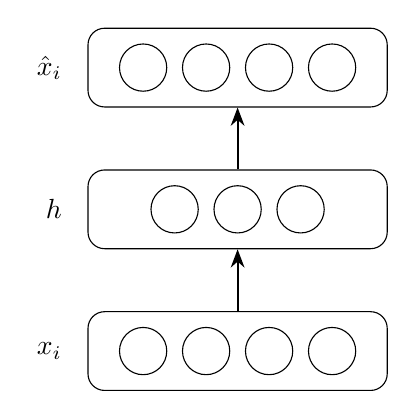
\begin{tikzpicture}[
		>=Stealth,
		neuron/.style={
			circle,
			draw,
			minimum size=6mm,
			inner sep=0pt
		},
		layer/.style={
			draw,
			rounded corners=6pt,
			minimum width=3.8cm,
			minimum height=1.0cm
		}
		]
		
		% Input layer
		\node[layer] (input) at (0,0) {};
		\foreach \x in {-1.2,-0.4,0.4,1.2}
		\node[neuron] at ([xshift=\x cm]input.center) {};
		
		% Hidden layer
		\node[layer] (hidden) at (0,1.8) {};
		\foreach \x in {-0.8,0,0.8}
		\node[neuron] at ([xshift=\x cm]hidden.center) {};
		
		% Output layer
		\node[layer] (output) at (0,3.6) {};
		\foreach \x in {-1.2,-0.4,0.4,1.2}
		\node[neuron] at ([xshift=\x cm]output.center) {};
		
		% Connections
		\draw[->,thick] (input.north) -- (hidden.south);
		\draw[->,thick] (hidden.north) -- (output.south);
		
		\node[left=0.2cm of input] {$x_i$};
		\node[left=0.2cm of hidden] {$h$};
		\node[left=0.2cm of output] {$\hat{x}_i$};
		
	\end{tikzpicture}
	\caption{Autoencoder representation}
\end{figure}


\[
\underbrace{
	\begin{bmatrix}
		0&0&0&\cdots&0
	\end{bmatrix}
}_{x_i}
\]

For MNIST data,

\[
|x_i|=28\times28=784.
\]

Therefore,

\[
x_i\in\mathbb{R}^{784}.
\]

Suppose the hidden representation is

\[
h\in\mathbb{R}^{d},
\]

where

\[
d<784.
\]

Thus, the autoencoder learns a lower-dimensional representation of
the input data.

\begin{figure}[H]
	\centering
	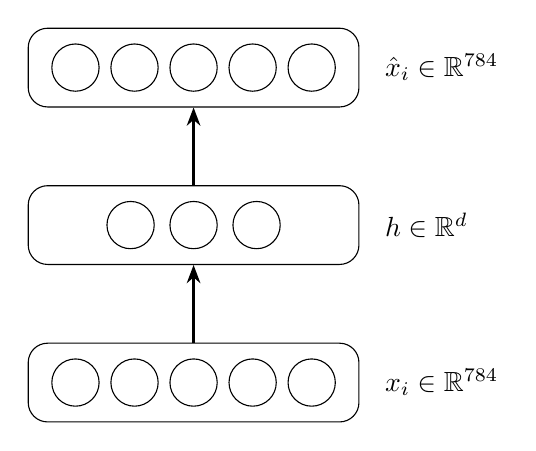
\begin{tikzpicture}[
		>=Stealth,
		neuron/.style={
			circle,
			draw,
			minimum size=6mm,
			inner sep=0pt
		},
		layer/.style={
			draw,
			rounded corners=7pt,
			minimum width=4.2cm,
			minimum height=1.0cm
		}
		]
		
		% Input
		\node[layer] (input) at (0,0) {};
		\foreach \x in {-1.5,-0.75,0,0.75,1.5}
		\node[neuron] at ([xshift=\x cm]input.center) {};
		
		% Hidden
		\node[layer] (hidden) at (0,2) {};
		\foreach \x in {-0.8,0,0.8}
		\node[neuron] at ([xshift=\x cm]hidden.center) {};
		
		% Output
		\node[layer] (output) at (0,4) {};
		\foreach \x in {-1.5,-0.75,0,0.75,1.5}
		\node[neuron] at ([xshift=\x cm]output.center) {};
		
		% Connections
		\draw[->,thick] (input.north) -- (hidden.south);
		\draw[->,thick] (hidden.north) -- (output.south);
		
		\node[right=0.2cm of input] {$x_i\in\mathbb{R}^{784}$};
		\node[right=0.2cm of hidden] {$h\in\mathbb{R}^{d}$};
		\node[right=0.2cm of output] {$\hat{x}_i\in\mathbb{R}^{784}$};
		
	\end{tikzpicture}
	\caption{Dimensionality reduction using an autoencoder}
\end{figure}


%%%%%%%%%%%%%%%%%%%%%%%%%%%%%%%%%%%%%%%%%%%%%%%%%%%%%%%%%%%%%%%%%%%%
% PAGE 2
%%%%%%%%%%%%%%%%%%%%%%%%%%%%%%%%%%%%%%%%%%%%%%%%%%%%%%%%%%%%%%%%%%%%

\subsection{Hidden Feature Representation}

What happens here, we know the input data, and we have perfect feature
representation which exactly captures the data.

Our original aim was to do classification.

So what we need to do?

We keep the first few layers of the autoencoder and throw away the
last layer.

\begin{figure}[H]
	\centering
	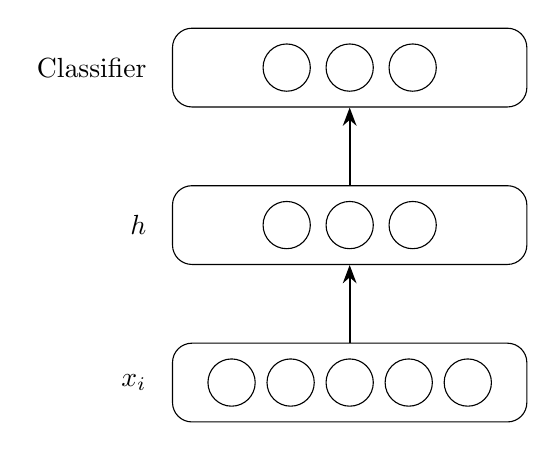
\begin{tikzpicture}[
		>=Stealth,
		layer/.style={
			draw,
			rounded corners=7pt,
			minimum width=4.5cm,
			minimum height=1.0cm
		},
		neuron/.style={
			circle,
			draw,
			minimum size=6mm,
			inner sep=0pt
		}
		]
		
		% Input
		\node[layer] (input) at (0,0) {};
		\foreach \x in {-1.5,-0.75,0,0.75,1.5}
		\node[neuron] at ([xshift=\x cm]input.center) {};
		
		% Hidden
		\node[layer] (hidden) at (0,2) {};
		\foreach \x in {-0.8,0,0.8}
		\node[neuron] at ([xshift=\x cm]hidden.center) {};
		
		% Classification layer
		\node[layer] (class) at (0,4) {};
		\foreach \x in {-0.8,0,0.8}
		\node[neuron] at ([xshift=\x cm]class.center) {};
		
		\draw[->,thick] (input.north) -- (hidden.south);
		\draw[->,thick] (hidden.north) -- (class.south);
		
		\node[left=0.2cm of input] {$x_i$};
		\node[left=0.2cm of hidden] {$h$};
		\node[left=0.2cm of class] {Classifier};
		
	\end{tikzpicture}
	\caption{Using learned hidden features for classification}
\end{figure}

We can learn hidden feature value from AE, and feed the feature layer
to the classifier.

\[
\underbrace{
	\begin{bmatrix}
		0&0&0&0&0
	\end{bmatrix}
}_{\text{input}}
\]

\[
\underbrace{
	\begin{bmatrix}
		0&0&0
	\end{bmatrix}
}_{\text{hidden feature}}
\]

For example,

\[
h_i=\sigma(w_i^T x_i),
\]

where \(w_i\) is the shared vector of weights connecting the input to
the hidden layer.

What values of \(x_i\) will cause \(h_i\) to be maximum
(or maximally activated)?

Suppose we assume that our inputs are normalized such that

\[
\|x_i\|=1.
\]

So, we are interested to solve the following:

\[
\max_{x_i}\; w_i^T x_i
\]

subject to

\[
\|x_i\|^2=x_i^T x_i=1.
\]

The product is maximized when both vectors are in the same direction.

Therefore,

\[
x_i=
\frac{w_i}{\sqrt{w_i^T w_i}}.
\]

Thus, the input which maximally activates the hidden neuron is

\[
\boxed{
	x_i=
	\frac{w_i}{\sqrt{w_i^T w_i}}
}
\]

Hence,

\[
q_i=
\frac{w_1}{\sqrt{w_1^Tw_1}},
\qquad
\frac{w_2}{\sqrt{w_2^Tw_2}},
\qquad
\cdots,
\qquad
\frac{w_n}{\sqrt{w_n^Tw_n}}.
\]

will respectively cause hidden neurons \(1\) to \(n\) to maximally
fire.


%%%%%%%%%%%%%%%%%%%%%%%%%%%%%%%%%%%%%%%%%%%%%%%%%%%%%%%%%%%%%%%%%%%%
% PAGE 3
%%%%%%%%%%%%%%%%%%%%%%%%%%%%%%%%%%%%%%%%%%%%%%%%%%%%%%%%%%%%%%%%%%%%

\subsection{Visualization of Learned Features}

Which hidden neuron will be learning the different shapes, as we
discuss, will be more clear for us with this visualization.

\begin{figure}[H]
	\centering
	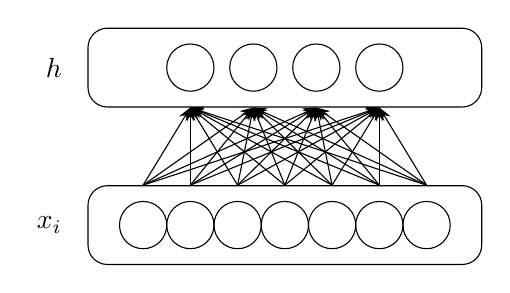
\begin{tikzpicture}[
		>=Stealth,
		layer/.style={
			draw,
			rounded corners=7pt,
			minimum width=5cm,
			minimum height=1.0cm
		},
		neuron/.style={
			circle,
			draw,
			minimum size=6mm,
			inner sep=0pt
		}
		]
		
		% Input
		\node[layer] (input) at (0,0) {};
		\foreach \x in {-1.8,-1.2,-0.6,0,0.6,1.2,1.8}
		\node[neuron] at ([xshift=\x cm]input.center) {};
		
		% Hidden
		\node[layer] (hidden) at (0,2) {};
		\foreach \x in {-1.2,-0.4,0.4,1.2}
		\node[neuron] at ([xshift=\x cm]hidden.center) {};
		
		% Connections
		\foreach \x in {-1.8,-1.2,-0.6,0,0.6,1.2,1.8}
		{
			\draw[->] 
			([xshift=\x cm]input.north)
			-- ([xshift=-1.2cm]hidden.south);
			
			\draw[->]
			([xshift=\x cm]input.north)
			-- ([xshift=-0.4cm]hidden.south);
			
			\draw[->]
			([xshift=\x cm]input.north)
			-- ([xshift=0.4cm]hidden.south);
			
			\draw[->]
			([xshift=\x cm]input.north)
			-- ([xshift=1.2cm]hidden.south);
		}
		
		\node[left=0.2cm of input] {$x_i$};
		\node[left=0.2cm of hidden] {$h$};
		
	\end{tikzpicture}
	\caption{Learned hidden features}
\end{figure}

We can learn hidden feature values from AE, and feed the feature layer
to the classifier.

\[
h_i=\sigma(w_i^T x_i).
\]

where \(w_i\) is the shared vector of weights connecting the input to
the hidden layer.

The different values of \(x_i\) will cause different hidden neurons to
be maximally activated.

Suppose we assume that our inputs are normalized so that

\[
\|x_i\|=1.
\]

We are interested to solve

\[
\max_{x_i}\{w_i^T x_i\}
\]

subject to

\[
\|x_i\|^2=x_i^Tx_i=1.
\]

So,

\[
x_i=
\frac{w_i}{\sqrt{w_i^Tw_i}}.
\]

Thus, inputs are

\[
q_i=
\frac{w_1}{\sqrt{w_1^Tw_1}},
\quad
\frac{w_2}{\sqrt{w_2^Tw_2}},
\quad
\cdots,
\quad
\frac{w_n}{\sqrt{w_n^Tw_n}}.
\]

These will respectively cause hidden neurons \(1\) to \(n\) to
maximally fire.

%%%%%%%%%%%%%%%%%%%%%%%%%%%%%%%%%%%%%%%%%%%%%%%%%%%%%%%%%%%%%%%%%%%%




%=========================================================
% Bias and Variance
%=========================================================

\section*{Bias and Variance}

\begin{itemize}
	\item We sample 25 points from training data and train a simple and a complex model.
	
	\item We repeat this process 25 times, i.e., train multiple models (each made from a different sample of the training data).
	
	\item We are trying to learn the parameter values of the training data.
	
	\item The parameter value will change, when we use different samples.
\end{itemize}

\begin{center}
	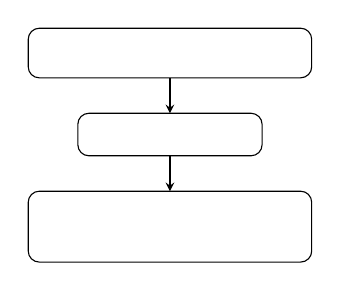
\begin{tikzpicture}[>=stealth,scale=0.9]
		
		% First model
		\draw[rounded corners] (-2,3) rectangle (2,3.7);
		\draw[->] (0,3) -- (0,2.5);
		
		% Second model
		\draw[rounded corners] (-1.3,1.9) rectangle (1.3,2.5);
		\draw[->] (0,1.9) -- (0,1.4);
		
		% Third model
		\draw[rounded corners] (-2,0.4) rectangle (2,1.4);
		
	\end{tikzpicture}
\end{center}

\noindent
We consider the problem of fitting a curve from a given set of training points.

\begin{itemize}
	\item We consider two models:
\end{itemize}

\[
y = wx+w_0
\]

\[
y = f(x)=\sum_{i=1}^{n}w_i x^i+w_0
\]

\begin{center}
	\begin{tikzpicture}[>=stealth,scale=0.9]
		
		% simple model
		\begin{axis}[
			width=6cm,
			height=4.5cm,
			axis lines=middle,
			xmin=0,xmax=10,
			ymin=0,ymax=10,
			xtick=\empty,
			ytick=\empty
			]
			\addplot[domain=0:10,samples=100] {0.65*x+1};
		\end{axis}
		
		% complex model
		\begin{axis}[
			at={(7cm,0)},
			width=6cm,
			height=4.5cm,
			axis lines=middle,
			xmin=0,xmax=10,
			ymin=0,ymax=10,
			xtick=\empty,
			ytick=\empty
			]
			\addplot[domain=0:10,samples=100] 
			{4+2*sin(deg(x))+0.3*sin(deg(3*x))};
		\end{axis}
		
	\end{tikzpicture}
\end{center}

%=========================================================
% Training samples
%=========================================================

\begin{itemize}
	\item We sample 25 points from training data and train a simple and a complex model.
	
	\item We repeat this process $n$ times.
	
	\item We train multiple models (each made from a different sample of the training data).
	
	\item We are trying to learn the parameter value of the training data.
\end{itemize}

\begin{center}
	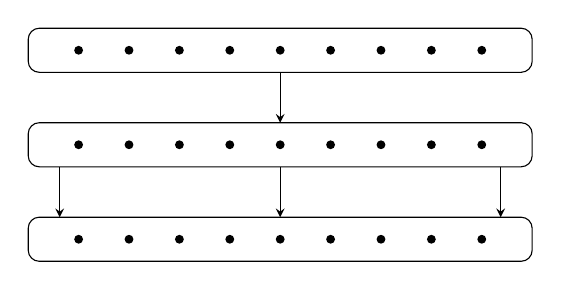
\begin{tikzpicture}[>=stealth,scale=0.8]
		
		% Original sample
		\draw[rounded corners] (-4,2.5) rectangle (4,3.2);
		\foreach \x in {-3.2,-2.4,-1.6,-0.8,0,0.8,1.6,2.4,3.2}
		\fill (\x,2.85) circle (2pt);
		
		% sample after training
		\draw[rounded corners] (-4,1) rectangle (4,1.7);
		\foreach \x in {-3.2,-2.4,-1.6,-0.8,0,0.8,1.6,2.4,3.2}
		\fill (\x,1.35) circle (2pt);
		
		\draw[->] (0,2.5) -- (0,1.7);
		
		% model
		\draw[rounded corners] (-4,-0.5) rectangle (4,0.2);
		\foreach \x in {-3.2,-2.4,-1.6,-0.8,0,0.8,1.6,2.4,3.2}
		\fill (\x,-0.15) circle (2pt);
		
		\draw[->] (-3.5,1) -- (-3.5,0.2);
		\draw[->] (0,1) -- (0,0.2);
		\draw[->] (3.5,1) -- (3.5,0.2);
		
	\end{tikzpicture}
\end{center}

%=========================================================
% High variance
%=========================================================

\section*{(high variance)}

\begin{itemize}
	\item What is happening here, due high no. of parameters, there is a tendency to overfit, so when we change the sample data points the output function are very different from each other.
\end{itemize}

\begin{center}
	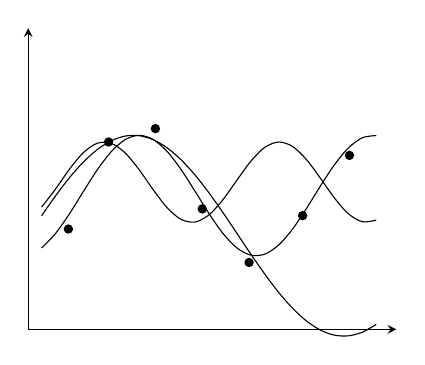
\begin{tikzpicture}[>=stealth,scale=0.85]
		
		\draw[->] (0,0) -- (5.5,0);
		\draw[->] (0,0) -- (0,4.5);
		
		% different fitted curves
		\draw[domain=0.2:5.2,smooth] plot (\x,{1.4+1.5*sin(deg(1.0*\x))});
		\draw[domain=0.2:5.2,smooth] plot (\x,{2.0+0.9*sin(deg(1.8*\x+30))});
		\draw[domain=0.2:5.2,smooth] plot (\x,{2.2+0.6*sin(deg(2.4*\x-20))});
		
		% points
		\foreach \x/\y in {
			0.6/1.5,
			1.2/2.8,
			1.9/3.0,
			2.6/1.8,
			3.3/1.0,
			4.1/1.7,
			4.8/2.6
		}
		\fill (\x,\y) circle (2pt);
		
	\end{tikzpicture}
\end{center}

%=========================================================
% Statistical concepts
%=========================================================

\noindent
Now let us derive few concepts from statistics.

\begin{itemize}
	\item Let $f(n)$ be the true model (sinusoidal in this case) and
	$\hat{f}(n)$ be our estimate of the model (simple or complex, in this case) then
\end{itemize}

\[
\operatorname{Bias}\left(\hat{f}(n)\right)
=
E\left[\hat{f}(n)\right]-f(n)
\]

\begin{center}
	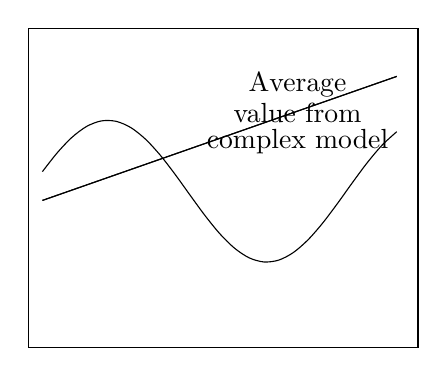
\begin{tikzpicture}[>=stealth,scale=0.9]
		
		\draw (0,0) rectangle (5.5,4.5);
		
		% simple model
		\draw[domain=0.2:5.2,smooth]
		plot (\x,{2.0+0.35*\x});
		
		% true model
		\draw[domain=0.2:5.2,smooth]
		plot (\x,{2.2+1.0*sin(deg(1.4*\x))});
		
		% average value
		\draw[domain=0.2:5.2,smooth]
		plot (\x,{2.0+0.35*\x});
		
		\node at (3.8,3.7) {Average};
		\node at (3.8,3.3) {value from};
		\node at (3.8,2.9) {complex model};
		
	\end{tikzpicture}
\end{center}

%=========================================================
% Bias explanation
%=========================================================

\begin{itemize}
	\item Now, if we consider the straight line then we can say that our bias is very high.
	
	\item $E[\hat{f}(n)]$ is the average (or expected) value of the model.
	
	\item We can see that for the simple model the average value (green line) is very far from the true value $f(n)$ (sinusoidal function).
	
	\item Mathematically, a simple model has a high bias.
\end{itemize}

%=========================================================
% Variance
%=========================================================

\begin{itemize}
	\item What is happening here, due high no. of parameters, there is a tendency to overfit, so when we change the sample data points the output functions are very different from each other.
\end{itemize}

\begin{center}
	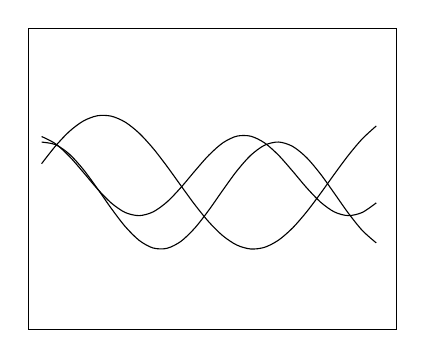
\begin{tikzpicture}[>=stealth,scale=0.85]
		
		\draw (0,0) rectangle (5.5,4.5);
		
		% Several curves
		\draw[domain=0.2:5.2,smooth]
		plot (\x,{2.2+1.0*sin(deg(1.4*\x))});
		
		\draw[domain=0.2:5.2,smooth]
		plot (\x,{2.0+0.8*sin(deg(1.8*\x+20))});
		
		\draw[domain=0.2:5.2,smooth]
		plot (\x,{2.3+0.6*sin(deg(2.0*\x-30))});
		
	\end{tikzpicture}
\end{center}


We now define variance:

\[
\operatorname{Variance}\left(\hat{f}(x)\right)
=
E\left[
\left(
\hat{f}(x)-E[\hat{f}(x)]
\right)^2
\right]
\]

\begin{itemize}
	
	\item Roughly speaking, it tells us how much the difference of $\hat{f}(x)$ is
	determined on different samples of the data differ from each other.
	
	\item It is clear that the simple model has a low variance whereas the
	complex model has a high variance.
	
\end{itemize}

\begin{center}
	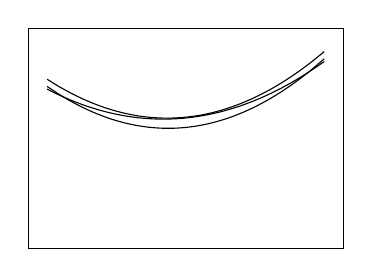
\begin{tikzpicture}[scale=0.8]
		
		\draw (0,0) rectangle (5,3.5);
		
		\draw[domain=0.3:4.7,smooth]
		plot (\x,{2.8-0.8*\x+0.18*\x*\x});
		
		\draw[domain=0.3:4.7,smooth]
		plot (\x,{2.7-0.6*\x+0.14*\x*\x});
		
		\draw[domain=0.3:4.7,smooth]
		plot (\x,{2.9-0.75*\x+0.17*\x*\x});
		
	\end{tikzpicture}
\end{center}

\begin{itemize}
	
	\item Simple model: high bias, low variance
	
	\item Complex model: low bias, high variance
	
	\item There is always a trade-off between bias and variance.
	
	\item Both bias and variance contribute to the overall prediction error.
	
\end{itemize}


\section*{Train error VS. Test error}

\begin{itemize}[leftmargin=1.2cm]
	\item Consider a new point $(x,y)$ which was not seen during training.
	
	\item If we use the model $\hat{f}(x)$ to predict the value of $y$, then
	the mean square error is given by
	\[
	\mathbb{E}\left[(y-\hat{f}(x))^2\right].
	\]
	
	Every time we get a new training point, hence it can be considered
	as random.
\end{itemize}

We can show that
\[
\boxed{
	\mathbb{E}\left[(y-\hat{f}(x))^2\right]
	=
	\operatorname{Bias}^2
	+
	\operatorname{Variance}
	+
	\sigma^2
	\quad
	\text{(irreducible error)}
}
\]

\vspace{0.3cm}

\begin{center}
	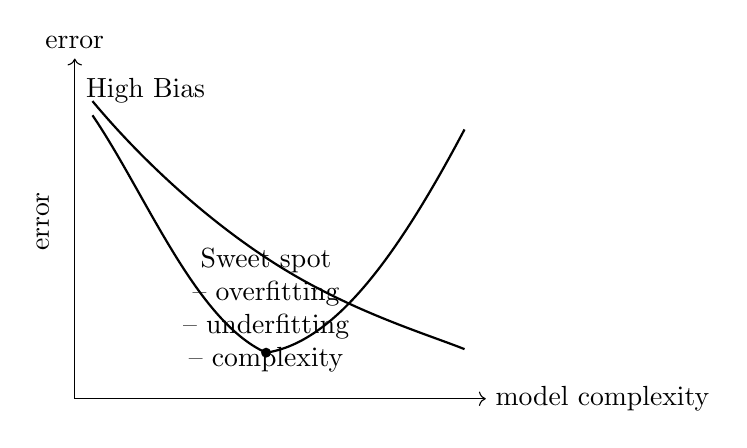
\begin{tikzpicture}[scale=0.9]
		
		% Axes
		\draw[->] (0,0) -- (5.8,0) node[right] {model complexity};
		\draw[->] (0,0) -- (0,4.8) node[above] {error};
		
		% High bias curve
		\draw[thick]
		(0.25,4.2)
		.. controls (1.0,3.3) and (2.0,2.4)
		.. (3.0,1.8)
		.. controls (4.0,1.2) and (5.0,0.9)
		.. (5.5,0.7);
		
		% Test error / U-shaped curve
		\draw[thick]
		(0.25,4.0)
		.. controls (1.0,2.9) and (1.7,1.1)
		.. (2.7,0.65)
		.. controls (3.7,0.8) and (4.6,2.1)
		.. (5.5,3.8);
		
		% Sweet spot
		\fill (2.7,0.65) circle (2pt);
		\node[align=center] at (2.7,1.25)
		{Sweet spot\\
			-- overfitting\\
			-- underfitting\\
			-- complexity};
		
		\node[rotate=90] at (-0.45,2.5) {error};
		
		\node at (1.0,4.35) {High Bias};
		
	\end{tikzpicture}
\end{center}

\begin{itemize}[leftmargin=1.2cm]
	\item The parameters of $\hat{f}(x)$ (all $w_i$'s) are trained using a
	training set
	\[
	\{(x_i,y_i)\}_{i=1}^{n}.
	\]
	
	\item However, at test time we are interested in evaluating the model
	on a validation (unseen) set which has not been used for training.
	
	\item This gives rise to the following two entities of interest:
	\begin{itemize}
		\item train error (say, mean square error)
		\item test error
	\end{itemize}
\end{itemize}

\newpage

% ============================================================
% PAGE 2
% ============================================================

\begin{itemize}[leftmargin=1.2cm]
	
	\item Let there be $n$ training points and $m$ test (validation) points.
	
\end{itemize}

\[
\boxed{
	\mathrm{Train}_{err}
	=
	\frac{1}{n}
	\sum_{i=1}^{n}
	\left(y_i-\hat{f}(x_i)\right)^2
}
\]

\[
\boxed{
	\mathrm{Test}_{err}
	=
	\frac{1}{m}
	\sum_{i=n+1}^{n+m}
	\left(y_i-\hat{f}(x_i)\right)^2
}
\]

\begin{itemize}[leftmargin=1.2cm]
	
	\item As model complexity increases, train error becomes overly
	optimistic and gives us a wrong picture of how close $\hat{f}$ is to $f$.
	
	\item The validation error gives the real picture of how $\hat{f}$ is to
	$f$.
	
\end{itemize}

\vspace{0.3cm}

\begin{center}
	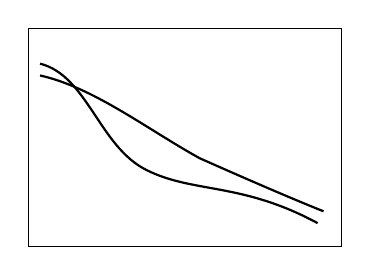
\begin{tikzpicture}[scale=0.75]
		
		\draw (0,0) rectangle (5.3,3.7);
		
		\draw[thick]
		(0.2,3.1)
		.. controls (1.0,2.9) and (1.2,1.7)
		.. (2.0,1.3)
		.. controls (2.8,0.9) and (3.6,1.1)
		.. (4.9,0.4);
		
		\draw[thick]
		(0.2,2.9)
		.. controls (1.1,2.7) and (2.0,2.0)
		.. (2.9,1.5)
		.. controls (3.8,1.1) and (4.5,0.8)
		.. (5.0,0.6);
		
	\end{tikzpicture}
\end{center}

\begin{itemize}[leftmargin=1.2cm]
	
	\item Let
	\[
	D=\{(x_i,y_i)\}_{i=1}^{n+m}.
	\]
	Then for any point $(x_i,y_i)$ we have
	\[
	y_i=f(x_i)+\epsilon_i.
	\]
	
	\item which means that $y_i$ is related to $x_i$ by some same function.
	
	\item Both have the same $f$ but there is also same noise $\epsilon$ in
	the regression.
	
	\item For simplicity, we assume
	\[
	\epsilon\sim\mathcal{N}(0,\sigma^2).
	\]
	
\end{itemize}

\newpage

% ============================================================
% PAGE 3
% ============================================================

\begin{itemize}[leftmargin=1.2cm]
	
	\item Further, we use $\hat{f}$ to approximate $f$ and estimate the
	parameter using T.C.D such that
	\[
	\hat{y}_i=\hat{f}(x_i).
	\]
	
\end{itemize}

We interested in knowing
\[
\boxed{
	\mathbb{E}\left[
	\left(\hat{f}(x_i)-f(x_i)\right)^2
	\right]
}
\]

but we cannot estimate this directly because we do not know $f$.

\begin{itemize}[leftmargin=1.2cm]
	\item We will see how to estimate this empirically using the observation
	$\hat{y}_i$ to prediction $\hat{y}_i$.
\end{itemize}

Since
\[
y_i=f(x_i)+\epsilon_i,
\]
we have

\begin{align*}
	\mathbb{E}\left[(\hat{y}_i-y_i)^2\right]
	&=
	\mathbb{E}\left[
	\left(
	\hat{f}(x_i)-f(x_i)-\epsilon_i
	\right)^2
	\right]
	\\[4pt]
	&=
	\mathbb{E}\left[
	\left(\hat{f}(x_i)-f(x_i)\right)^2
	-2\epsilon_i
	\left(\hat{f}(x_i)-f(x_i)\right)
	+\epsilon_i^2
	\right]
	\\[4pt]
	&=
	\mathbb{E}\left[
	\left(\hat{f}(x_i)-f(x_i)\right)^2
	\right]
	\\
	&\qquad
	-2\mathbb{E}\left[
	\epsilon_i
	\left(\hat{f}(x_i)-f(x_i)\right)
	\right]
	+\mathbb{E}\left[\epsilon_i^2\right].
\end{align*}

Therefore,

\[
\boxed{
	\mathbb{E}\left[
	\left(\hat{f}(x_i)-f(x_i)\right)^2
	\right]
	=
	\mathbb{E}\left[
	(\hat{y}_i-y_i)^2
	\right]
	-
	\mathbb{E}[\epsilon_i^2]
	+
	2\mathbb{E}\left[
	\epsilon_i
	\left(\hat{f}(x_i)-f(x_i)\right)
	\right]
}
\tag{1}
\]

\vspace{0.3cm}

\begin{center}
	\begin{tikzpicture}[scale=0.8]
		
		\draw[->] (0,0) -- (5.4,0) node[right] {$x$};
		\draw[->] (0,0) -- (0,4.0) node[above] {$y$};
		
		\draw[thick]
		(0.3,1.0)
		.. controls (1.0,3.0) and (2.0,3.4)
		.. (2.7,2.0)
		.. controls (3.3,0.8) and (4.2,0.6)
		.. (5.0,2.5);
		
		\draw[dashed]
		(0.3,1.4) -- (5.0,1.4);
		
	\end{tikzpicture}
\end{center}

\newpage

% ============================================================
% PAGE 4
% ============================================================

\[
\boxed{
	\mathbb{E}\left[(\hat{y}_i-y_i)^2\right]
	=
	\frac{1}{m}
	\sum_{i=n+1}^{n+m}
	(\hat{y}_i-y_i)^2
}
\]

\hfill
\textit{Empirical because, min is the only way we can do.}

\vspace{0.4cm}

\underline{\textbf{case 1: Using test observation}}

\vspace{0.2cm}

\[
\mathbb{E}
\left[
\left(\hat{f}(x_i)-f(x_i)\right)^2
\right]
_{\text{true error}}
\]

\begin{align*}
	&=
	\frac{1}{m}
	\sum_{i=n+1}^{n+m}
	(\hat{y}_i-y_i)^2
	-
	\frac{1}{m}
	\sum_{i=n+1}^{n+m}
	\epsilon_i^2
	\\
	&\qquad
	+
	2\mathbb{E}
	\left[
	\epsilon_i
	\left(
	\hat{f}(x_i)-f(x_i)
	\right)
	\right].
\end{align*}

\vspace{0.3cm}

\[
\underbrace{
	\frac{1}{m}
	\sum_{i=n+1}^{n+m}
	(\hat{y}_i-y_i)^2
}_{\text{empirical estimate of error}}
\qquad
-
\qquad
\underbrace{
	\frac{1}{m}
	\sum_{i=n+1}^{n+m}
	\epsilon_i^2
}_{\text{small error}}
\]

\vspace{0.3cm}

\[
+
\;2\mathbb{E}
\left[
\epsilon_i
\left(
\hat{f}(x_i)-f(x_i)
\right)
\right]
\]

\begin{itemize}[leftmargin=1.2cm]
	
	\item $\epsilon_i$ is independent of other random variable we see in the
	expectation.
	
	\item None of the test observation participated in the estimation of
	$\hat{f}(x)$.
	
\end{itemize}

\[
\therefore\quad
\epsilon_i
\perp
\left(
\hat{f}(x_i)-f(x_i)
\right)
\]

\[
\therefore\quad
\mathbb{E}
\left[
\epsilon_i
\left(
\hat{f}(x_i)-f(x_i)
\right)
\right]
=
\mathbb{E}[\epsilon_i]\,
\mathbb{E}
\left[
\hat{f}(x_i)-f(x_i)
\right]
\]

\[
=0\cdot
\mathbb{E}
\left[
\hat{f}(x_i)-f(x_i)
\right]
=0
\]

\vspace{0.4cm}

\[
\boxed{
	\text{true error}
	=
	\text{empirical test error}
	+
	\text{small correction}
}
\]

\section{Training Error, Test Error, and Model Complexity}

\subsection{Training Error vs. Test Error}

Consider a new point $(x,y)$ which has not been seen during training. If we use the model $\hat{f}(x)$ to predict the value of $y$, the mean squared error is

\[
\mathbb{E}\left[(y-\hat{f}(x))^2\right].
\]

Every time we add a new training point, the model is retrained. Hence, the training points can be regarded as random observations.

Let the true relationship between $x$ and $y$ be

\[
y=f(x)+\epsilon,
\]

where $\epsilon$ is a random noise term with

\[
\mathbb{E}[\epsilon]=0,
\qquad
\operatorname{Var}(\epsilon)=\sigma^2.
\]

The expected squared prediction error can be decomposed as

\begin{align}
	\mathbb{E}\left[(y-\hat{f}(x))^2\right]
	&=
	\mathbb{E}\left[
	\left(f(x)+\epsilon-\hat{f}(x)\right)^2
	\right] \\
	&=
	\mathbb{E}\left[
	\left(\hat{f}(x)-f(x)\right)^2
	\right]
	+
	\mathbb{E}[\epsilon^2] \nonumber\\
	&\quad
	+2\mathbb{E}\left[
	\epsilon\left(f(x)-\hat{f}(x)\right)
	\right].
\end{align}

Since $\epsilon$ is independent of the training data and has zero mean,

\[
\mathbb{E}\left[
\epsilon\left(\hat{f}(x)-f(x)\right)
\right]
=
\mathbb{E}[\epsilon]\,
\mathbb{E}\left[
\hat{f}(x)-f(x)
\right]
=0.
\]

Therefore,

\begin{equation}
	\boxed{
		\mathbb{E}\left[(y-\hat{f}(x))^2\right]
		=
		\mathbb{E}\left[
		(\hat{f}(x)-f(x))^2
		\right]
		+\sigma^2
	}
\end{equation}

where $\sigma^2$ represents the irreducible error.

\subsection{Empirical Estimation of Test Error}

Suppose the test observations are

\[
D_{\mathrm{test}}
=
\{(x_i,y_i)\}_{i=1}^{m},
\]

where these observations were not used during training.

The empirical test error can be estimated as

\begin{equation}
	\widehat{E}_{\mathrm{test}}
	=
	\frac{1}{m}
	\sum_{i=1}^{m}
	(y_i-\hat{f}(x_i))^2.
\end{equation}

This provides an empirical estimate of

\[
\mathbb{E}\left[(y-\hat{f}(x))^2\right].
\]

The important point is that the test observations are independent of the observations used for estimating the parameters of $\hat{f}(x)$.

\subsection{Case 1: Test Observations}

For a test observation,

\[
y_i=f(x_i)+\epsilon_i,
\]

where $\epsilon_i$ is independent of the training data.

Thus,

\begin{align}
	\mathbb{E}\left[
	\left(\hat{f}(x_i)-f(x_i)\right)^2
	\right]
	&=
	\mathbb{E}\left[
	(\hat{y}_i-y_i)^2
	\right]
	-\mathbb{E}[\epsilon_i^2] \\
	&\quad
	+2\mathbb{E}\left[
	\epsilon_i
	\left(\hat{f}(x_i)-f(x_i)\right)
	\right].
\end{align}

Since

\[
\mathbb{E}[\epsilon_i]=0
\]

and $\epsilon_i$ is independent of $\hat{f}(x_i)$,

\[
\mathbb{E}\left[
\epsilon_i
\left(\hat{f}(x_i)-f(x_i)\right)
\right]=0.
\]

Therefore,

\begin{equation}
	\boxed{
		\text{True error}
		=
		\text{Empirical test error}
		-\text{Irreducible error}
	}
\end{equation}

up to sampling variation.

\subsection{Case 2: Training Observations}

Now consider a training observation. The same observations used to estimate the parameters of $\hat{f}(x)$ are also used to calculate the error.

The expected squared error can be written as

\begin{equation}
	\mathbb{E}
	\left[
	\left(\hat{f}(x_i)-f(x_i)\right)^2
	\right]
	=
	\frac{1}{n}
	\sum_{i=1}^{n}
	(\hat{y}_i-y_i)^2
	-
	\frac{1}{n}
	\sum_{i=1}^{n}\epsilon_i^2
	+
	2\mathbb{E}
	\left[
	\epsilon_i
	\left(\hat{f}(x_i)-f(x_i)\right)
	\right].
\end{equation}

Unlike the test-error case,

\[
\epsilon_i
\not\!\perp\!\!\!\perp
\hat{f}(x_i),
\]

because the same observation is used for estimating $\hat{f}$.

Consequently,

\begin{equation}
	\mathbb{E}
	\left[
	\epsilon_i
	\left(\hat{f}(x_i)-f(x_i)\right)
	\right]
	\neq
	\mathbb{E}[\epsilon_i]\,
	\mathbb{E}
	\left[
	\hat{f}(x_i)-f(x_i)
	\right].
\end{equation}

Hence, the empirical training error is generally smaller than the true prediction error and does not provide an unbiased estimate of the error on unseen observations.

\subsection{True Error and Model Complexity}

As the complexity of a model increases, the model becomes more flexible and can fit the training data more closely.

For a simple model, the training error is relatively high. As model complexity increases, the training error generally decreases.

However, the test error behaves differently. Initially, increasing model complexity reduces the test error because the model becomes capable of capturing important patterns in the data. After a certain point, excessive complexity causes the model to fit noise in the training data, resulting in overfitting.

Thus, the test error typically has a U-shaped relationship with model complexity.

\begin{center}
	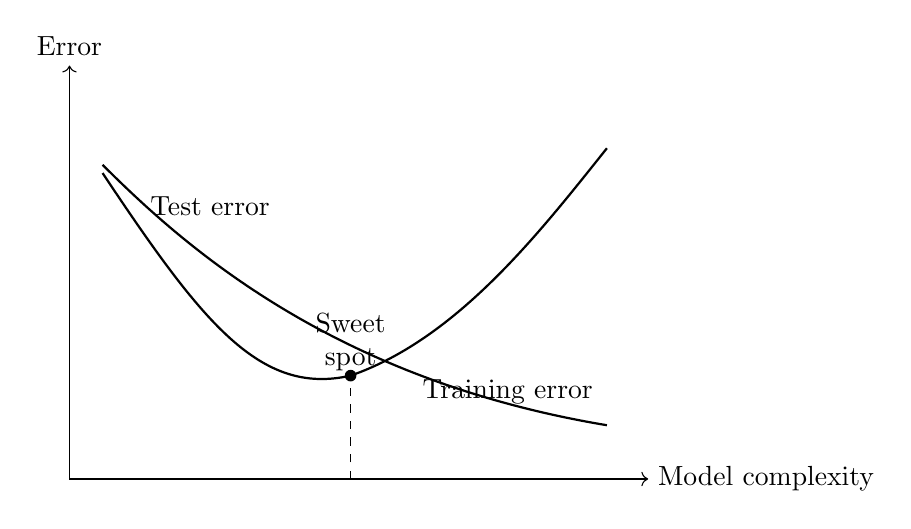
\begin{tikzpicture}[scale=1.05]
		
		% Axes
		\draw[->] (0,0) -- (7,0)
		node[right] {Model complexity};
		\draw[->] (0,0) -- (0,5)
		node[above] {Error};
		
		% Training error
		\draw[thick]
		(0.4,3.8)
		.. controls (1.4,2.8) and (3.2,1.2) ..
		(6.5,0.65);
		
		% Test error
		\draw[thick]
		(0.4,3.7)
		.. controls (1.6,1.9) and (2.3,1.0) ..
		(3.4,1.25)
		.. controls (4.7,1.7) and (5.7,3.0) ..
		(6.5,4.0);
		
		% Sweet spot
		\draw[dashed] (3.4,0) -- (3.4,1.25);
		\fill (3.4,1.25) circle (2pt);
		
		\node[align=center] at (3.4,1.65) {Sweet\\spot};
		
		\node at (1.7,3.3) {Test error};
		\node at (5.3,1.05) {Training error};
		
	\end{tikzpicture}
\end{center}

The point corresponding to the minimum test error represents the desirable level of model complexity. This point is sometimes referred to as the \emph{sweet spot}.

The relationship can therefore be summarized as

\begin{equation}
	\boxed{
		\text{True Error}
		=
		\text{Empirical Training Error}
		+
		\text{Estimation Error}
		+
		\Omega(\text{Model Complexity})
	}
\end{equation}

where $\Omega(\cdot)$ represents a penalty associated with model complexity.

\subsection{Stein's Lemma and Model Complexity}

Stein's lemma provides a connection between the sensitivity of the fitted model to the observations and the model's effective complexity.

For observations

\[
y_i=f(x_i)+\epsilon_i,
\qquad
\epsilon_i\sim\mathcal{N}(0,\sigma^2),
\]

the following quantity is related to the optimism of the training error:

\begin{equation}
	\frac{1}{n}
	\sum_{i=1}^{n}
	\mathbb{E}
	\left[
	\epsilon_i
	\left(
	\hat{f}(x_i)-f(x_i)
	\right)
	\right]
	=
	\frac{\sigma^2}{n}
	\sum_{i=1}^{n}
	\mathbb{E}
	\left[
	\frac{\partial \hat{f}(x_i)}
	{\partial y_i}
	\right].
\end{equation}

The quantity

\begin{equation}
	\boxed{
		\frac{\partial \hat{f}(x_i)}{\partial y_i}
	}
\end{equation}

measures how sensitive the fitted prediction is to a small change in the corresponding observation $y_i$.

A highly complex model tends to be more sensitive to changes in individual observations, whereas a simple model is generally less sensitive.

\subsection{Regularization and Model Complexity}

The above discussion provides the basis for regularization methods.

Regularization introduces an additional penalty term into the training objective:

\begin{equation}
	\boxed{
		\min_{\theta}
		\left[
		L(\theta)
		+
		\Omega(\theta)
		\right]
	}
\end{equation}

where

\begin{itemize}
	\item $L(\theta)$ is the training loss,
	\item $\theta$ represents the model parameters, and
	\item $\Omega(\theta)$ is the regularization penalty.
\end{itemize}

The purpose of regularization is to discourage unnecessarily complex models and thereby improve generalization.

For example, in $L_2$ regularization,

\begin{equation}
	\Omega(\theta)
	=
	\lambda
	\sum_j \theta_j^2,
\end{equation}

while for $L_1$ regularization,

\begin{equation}
	\Omega(\theta)
	=
	\lambda
	\sum_j |\theta_j|.
\end{equation}

Here, $\lambda$ controls the strength of regularization.

The regularized objective can therefore be written as

\begin{equation}
	\boxed{
		\theta^*
		=
		\arg\min_{\theta}
		\left\{
		L(\theta)+\lambda\Omega(\theta)
		\right\}.
	}
\end{equation}

For complex models, a stronger penalty is generally desirable, whereas simpler models require less regularization.

\begin{center}
	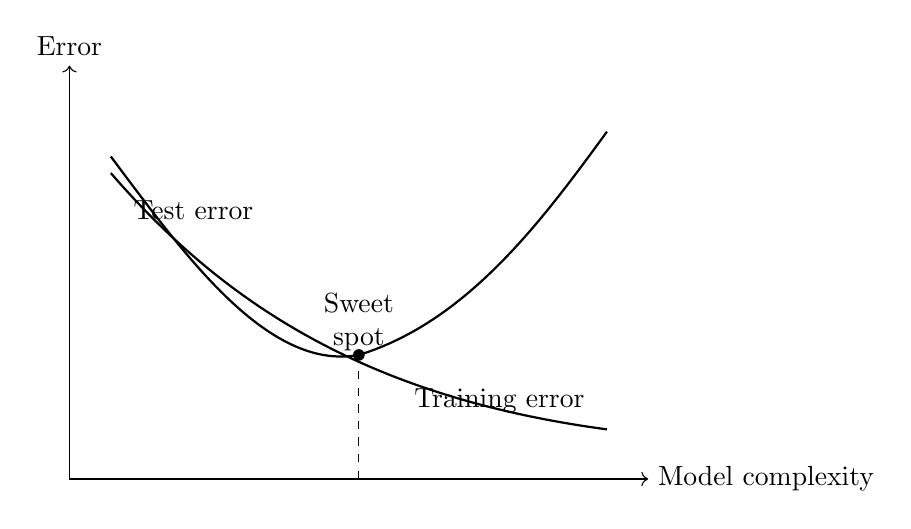
\begin{tikzpicture}[scale=1.05]
		
		% Axes
		\draw[->] (0,0) -- (7,0)
		node[right] {Model complexity};
		\draw[->] (0,0) -- (0,5)
		node[above] {Error};
		
		% Test error curve
		\draw[thick]
		(0.5,3.9)
		.. controls (1.4,2.7) and (2.4,1.3) ..
		(3.5,1.5)
		.. controls (4.8,1.9) and (5.7,3.1) ..
		(6.5,4.2);
		
		% Training error curve
		\draw[thick]
		(0.5,3.7)
		.. controls (1.8,2.2) and (3.5,1.0) ..
		(6.5,0.6);
		
		% Sweet spot
		\fill (3.5,1.5) circle (2pt);
		\draw[dashed] (3.5,0) -- (3.5,1.5);
		
		\node[align=center] at (3.5,1.9) {Sweet\\spot};
		
		\node at (1.5,3.25) {Test error};
		\node at (5.2,0.95) {Training error};
		
	\end{tikzpicture}
\end{center}

The regularization penalty should therefore be chosen so that the resulting model achieves an appropriate balance between fitting the training data and controlling model complexity.

In particular,

\begin{equation}
	\boxed{
		\text{Regularization}
		\quad\Longrightarrow\quad
		\text{lower effective model complexity}
		\quad\Longrightarrow\quad
		\text{better generalization}.
	}
\end{equation}

\end{document}
